% Options for packages loaded elsewhere
\PassOptionsToPackage{unicode}{hyperref}
\PassOptionsToPackage{hyphens}{url}
%
\documentclass[
  12pt,
]{book}
\usepackage{amsmath,amssymb}
\usepackage[]{kpfonts}
\usepackage{setspace}
\usepackage{iftex}
\ifPDFTeX
  \usepackage[T1]{fontenc}
  \usepackage[utf8]{inputenc}
  \usepackage{textcomp} % provide euro and other symbols
\else % if luatex or xetex
  \usepackage{unicode-math}
  \defaultfontfeatures{Scale=MatchLowercase}
  \defaultfontfeatures[\rmfamily]{Ligatures=TeX,Scale=1}
\fi
% Use upquote if available, for straight quotes in verbatim environments
\IfFileExists{upquote.sty}{\usepackage{upquote}}{}
\IfFileExists{microtype.sty}{% use microtype if available
  \usepackage[]{microtype}
  \UseMicrotypeSet[protrusion]{basicmath} % disable protrusion for tt fonts
}{}
\makeatletter
\@ifundefined{KOMAClassName}{% if non-KOMA class
  \IfFileExists{parskip.sty}{%
    \usepackage{parskip}
  }{% else
    \setlength{\parindent}{0pt}
    \setlength{\parskip}{6pt plus 2pt minus 1pt}}
}{% if KOMA class
  \KOMAoptions{parskip=half}}
\makeatother
\usepackage{xcolor}
\IfFileExists{xurl.sty}{\usepackage{xurl}}{} % add URL line breaks if available
\IfFileExists{bookmark.sty}{\usepackage{bookmark}}{\usepackage{hyperref}}
\hypersetup{
  pdftitle={Cours de mathématiques 1e},
  pdfauthor={Robinson Cartez},
  hidelinks,
  pdfcreator={LaTeX via pandoc}}
\urlstyle{same} % disable monospaced font for URLs
\usepackage{longtable,booktabs,array}
\usepackage{calc} % for calculating minipage widths
% Correct order of tables after \paragraph or \subparagraph
\usepackage{etoolbox}
\makeatletter
\patchcmd\longtable{\par}{\if@noskipsec\mbox{}\fi\par}{}{}
\makeatother
% Allow footnotes in longtable head/foot
\IfFileExists{footnotehyper.sty}{\usepackage{footnotehyper}}{\usepackage{footnote}}
\makesavenoteenv{longtable}
\usepackage{graphicx}
\makeatletter
\def\maxwidth{\ifdim\Gin@nat@width>\linewidth\linewidth\else\Gin@nat@width\fi}
\def\maxheight{\ifdim\Gin@nat@height>\textheight\textheight\else\Gin@nat@height\fi}
\makeatother
% Scale images if necessary, so that they will not overflow the page
% margins by default, and it is still possible to overwrite the defaults
% using explicit options in \includegraphics[width, height, ...]{}
\setkeys{Gin}{width=\maxwidth,height=\maxheight,keepaspectratio}
% Set default figure placement to htbp
\makeatletter
\def\fps@figure{htbp}
\makeatother
\setlength{\emergencystretch}{3em} % prevent overfull lines
\providecommand{\tightlist}{%
  \setlength{\itemsep}{0pt}\setlength{\parskip}{0pt}}
\setcounter{secnumdepth}{5}
\usepackage{booktabs}

\usepackage{color}
\usepackage{framed}
\usepackage{geometry}

\setlength{\fboxsep}{.8em}
\newenvironment{defboxshaded}{
 \definecolor{shadecolor}{rgb}{0, 0, 0} %black
 \color{white}
 \begin{shaded}}
 {\end{shaded}}
% 
\usepackage[most]{tcolorbox}
\usepackage{tikz}
\newtcolorbox{defbox}{
  boxrule=0.2pt,
  colback=red!6!white,
  colframe=black,
  coltext=black,
  boxsep=5pt,
  arc=4pt}
%
\newtcolorbox{reglebox}{
  boxrule=0.2pt,
  colback=yellow!10!white,
  colframe=black,
  coltext=black,
  boxsep=5pt,
  arc=4pt}
%  
\newtcolorbox{cadre}{
  %colback=yellow,
  colframe=black,
  coltext=black,
  boxsep=5pt,
  arc=4pt}
%
%
\newcommand{\rbox}[1]{\tikz[baseline={(a.base)}]\node[draw=black,rounded corners=0.5ex,,inner sep=1pt](a){#1};}
%  
% Pour les paragraphes à deux colonnes
\newenvironment{cols}[1]{}{}
\newenvironment{col}[1]{\begin{minipage}{#1}\ignorespaces}{%
\end{minipage}
\ifhmode\unskip\fi
\aftergroup\useignorespacesandallpars}

\def\useignorespacesandallpars#1\ignorespaces\fi{%
#1\fi\ignorespacesandallpars}

\makeatletter
\def\ignorespacesandallpars{%
 \@ifnextchar\par
   {\expandafter\ignorespacesandallpars\@gobble}%
   {}%
}
\makeatother
%
% Pour pouvoir avoir une autre font
%\usepackage{lxfonts}
\usepackage{kpfonts}
\renewcommand*\familydefault{\sfdefault}
\ifLuaTeX
  \usepackage{selnolig}  % disable illegal ligatures
\fi
\usepackage[]{natbib}
\bibliographystyle{plainnat}

\title{Cours de mathématiques 1e}
\author{Robinson Cartez}
\date{2022-08-20}

\begin{document}
\maketitle

{
\setcounter{tocdepth}{1}
\tableofcontents
}
\setstretch{1.5}
\hypertarget{bienvenus}{%
\chapter*{Bienvenus}\label{bienvenus}}
\addcontentsline{toc}{chapter}{Bienvenus}

\begin{cadre}
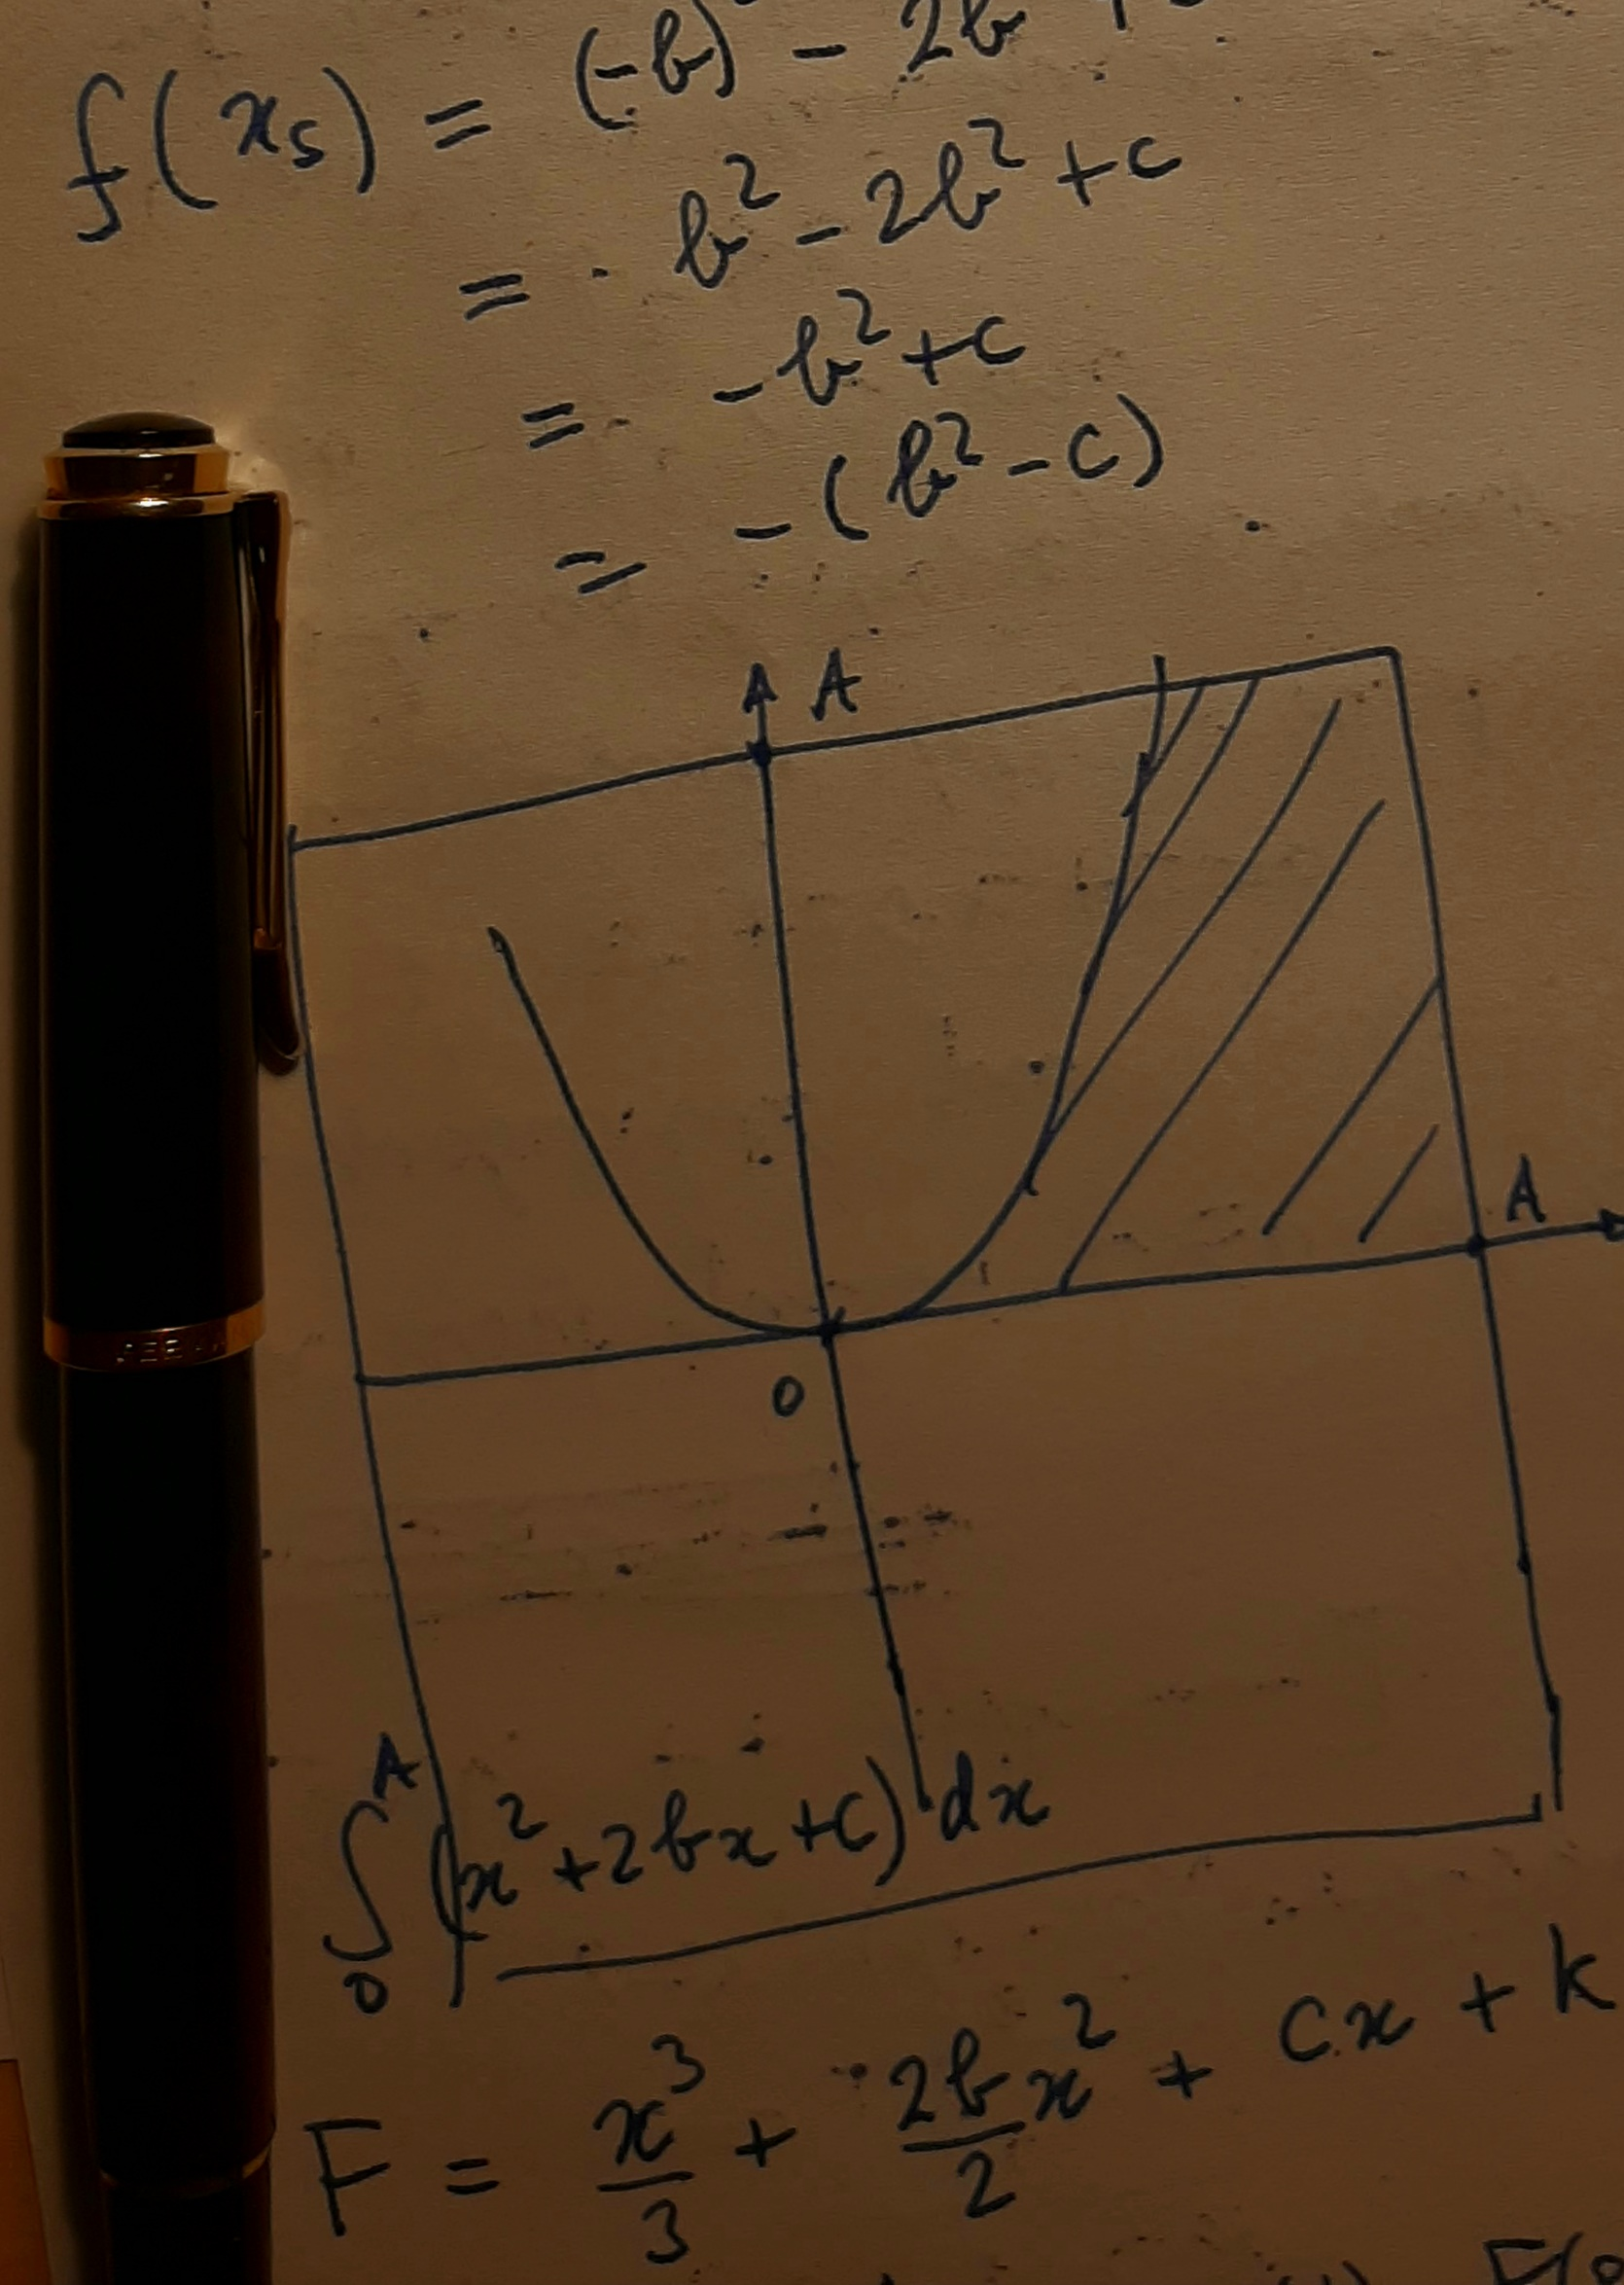
\includegraphics{images/cover_cours1e.jpg}

\end{cadre}

\hypertarget{liste-des-symboles-utilisuxe9s}{%
\chapter*{Liste des symboles utilisés}\label{liste-des-symboles-utilisuxe9s}}
\addcontentsline{toc}{chapter}{Liste des symboles utilisés}

\begin{longtable}[]{@{}
  >{\raggedright\arraybackslash}p{(\columnwidth - 2\tabcolsep) * \real{0.3750}}
  >{\raggedright\arraybackslash}p{(\columnwidth - 2\tabcolsep) * \real{0.6250}}@{}}
\toprule
\begin{minipage}[b]{\linewidth}\raggedright
Symbole
\end{minipage} & \begin{minipage}[b]{\linewidth}\raggedright
Description
\end{minipage} \\
\midrule
\endhead
\(\mathbb{N}\) & ensemble des nombres naturels \\
\(\mathbb{N}^*\) & ensemble des nombres naturels sans le zéro \\
\(\mathbb{Z}\) & ensemble des nombres entiers relatifs \\
\(\mathbb{Z}^*\) & ensemble des nombres entiers relatifs sans le zéro \\
\(\mathbb{Q}\) & ensemble des nombres rationnels \\
\(\mathbb{Q}^*\) & ensemble des nombres rationnels sans le zéro \\
\(\mathbb{Q}_+\) & ensemble des nombres rationnels positifs \\
\(\in\) & appartient à \\
\(\notin\) & n'appartient pas à \\
\(\subset\) & est inclus dans \\
\(\not\subset\) & est inclus dans \\
\(\cap\) & intersection \\
\(\cup\) & union \\
\(\varnothing\) ou \(\{\}\) & ensemble vide \\
\(<\) & inférieur à \\
\(>\) & supérieur à \\
\(\geq\) & supérieur ou égal à \\
\(\leq\) & inférieur ou égal à \\
\(\approx\) & approximativement égal à \\
\(=\) & égal à \\
\(\ne\) & n'est pas égal à \\
\(\infty\) & infini \\
\(+\infty\) & infini positifs \\
\(-\infty\) & infini négatifs \\
\(|\ldots|\) & valeur absolue de \(\ldots\) \\
\(\mapsto\) & a pour image \\
\(AB\) & segment nommé \(AB\) \\
\(\overline{AB}\) & longueur du segment \(AB\) \\
\([a;b]\) & intervalle fermé d'extrêmités \(a\) et \(b\) \\
\(]a;b[\) & intervalle ouvert d'extrêmités \(a\) et \(b\) \\
\(]a;b]\) & intervalle ouvert à gauche d'extrêmités \(a\) et \(b\) \\
\([a;b[\) & intervalle ouvert à droite d'extrêmités \(a\) et \(b\) \\
\(\alpha,~\beta,~\gamma,~\delta\) & mesures d'angle: alpha, beta, gamma, delta \\
\(d_1,~d_2,\ldots\) & droite 1, droite 2, etc. \\
\(//\) & est parallèle à \\
\(\perp\) & est perpendiculaire à \\
\(S=\{\ldots\}\) & ensemble des solutions d'une équation \\
\(\Leftrightarrow\) ou \(\Longleftrightarrow\) & ``si et seulement si'' ou ``équivalent'' \\
\(\Rightarrow\) ou \(\Longrightarrow\) & implique \\
\bottomrule
\end{longtable}

\hypertarget{semaine-1-calcul-littuxe9ral-1}{%
\chapter{Semaine 1 : Calcul littéral (1)}\label{semaine-1-calcul-littuxe9ral-1}}

\hypertarget{exemple-dintroduction}{%
\section{Exemple d'introduction}\label{exemple-dintroduction}}

D'après une légende arabe, le jeu d'échecs a été inventé par un
brahmane chargé de l'instruction d'un jeune roi.

Enthousiasmé par ce nouveau jeu, le roi offrit à l'inventeur la
récompense qu'il voudrait. Pour donner une nouvelle leçon à son élève,
le brahmane demanda un grain de blé sur la première case de
l'échiquier, deux sur la deuxième, quatre sur la troisième, huit sur
la quatrième, et ainsi de suite toujours en doublant le nombre de
grains de riz, jusqu'à la 64ème case et que le tout soit additionné et
lui fût remis.

D'apparence modeste, la demande fut accordée. Malheureusement, toutes les réserves de la terre ne purent y satisfaire.

En réalité, le roi aurait dû donner \(18446744073709551615\) grains de riz. Ceci correspond à environ \(1500\) ans de production mondiale actuelle.

Il est possible de noter le nombre de grains de riz de la manière suivante:

\begin{longtable}[]{@{}lcr@{}}
\toprule
Numéro case & Nombre de grains de riz & \\
\midrule
\endhead
\(1\) & \(1\) & \\
\(2\) & \(2\) & \\
\(3\) & \(2\cdot 2\) & \\
\(4\) & \((2\cdot 2)\cdot 2=2^3=8\) & \\
\(5\) & \((2\cdot 2\cdot 2)\cdot 2=2^4=16\) & \\
\(\cdots\) & \(\cdots\) & \\
\(64\) & \(2^{63}=9223372036854775808\) & \\
\bottomrule
\end{longtable}

\hypertarget{bases-thuxe9oriques}{%
\section{Bases théoriques}\label{bases-thuxe9oriques}}

\hypertarget{puissances}{%
\subsection{Puissances}\label{puissances}}

\begin{defbox}
On appelle \(\textbf{n}\) ième puissance de \(a\) un produit de \({\color{red}n}\) facteurs égaux à \(a\)

\[ a^n = \underbrace{a\cdot a\cdot \ldots \cdot a}_{n~\text{facteurs égaux à}~a}\]

\end{defbox}

\hypertarget{exemples}{%
\subsubsection{Exemples}\label{exemples}}

\[4^3=\underbrace{4\cdot 4\cdot 4}_{3~\text{facteurs égaux à}~4} = 64\]
\[b^4=\underbrace{b\cdot b\cdot b\cdot b}_{4~\text{facteurs égaux à}~b}\]

\hypertarget{signe-dune-puissance}{%
\subsection{Signe d'une puissance}\label{signe-dune-puissance}}

On utilise la règle des signes bien connue

\begin{reglebox}

\begin{enumerate}
\def\labelenumi{\arabic{enumi}.}
\tightlist
\item
  La puissance d'un nombre positif est toujours positive.
\item
  La puissance d'un nombre négatif est

  \begin{itemize}
  \tightlist
  \item
    \textbf{positive} si l'exposant est \textbf{pair}
  \item
    \textbf{négative} si l'exposant est \textbf{impair}
  \end{itemize}
\end{enumerate}

\end{reglebox}

\hypertarget{exemples-1}{%
\subsubsection{Exemples}\label{exemples-1}}

\begin{align*}
 (+7)^2 & = (+7)\cdot(+7) = +49 = 49\\
 (+5)^3 & = (+5)\cdot(+5)\cdot (+5) = +125 = 125\\
 (-3)^4 & = (-3)\cdot(-3)\cdot(-3)\cdot(-3) = -81\\
 (-2)^5 & = (-2)\cdot(-2)\cdot(-2)\cdot(-2)\cdot(-2) = -32\\
\end{align*}

\textbf{Remarque}
\[(-4)^2\neq -4^2\] mais \[(-4)^3 = -4^3\]

\hypertarget{produit-de-puissances-de-muxeame-base}{%
\subsection{Produit de puissances de même base}\label{produit-de-puissances-de-muxeame-base}}

\[a^2\cdot a^3=(a\cdot a)\cdot(a\cdot a\cdot a)=a\cdot a\cdot a\cdot a\cdot a\cdot = a^5 = a^{2+3}\]

On a donc la règle générale suivante pour deux exposants entiers \(n\) et \(m\)

\begin{reglebox}
Pour multiplier des puissances de \textbf{même base}, on conserve la base et on additionne les exposants.

\[a^n\cdot a^m = a^{n+m}\]

\end{reglebox}

\hypertarget{exemples-2}{%
\subsubsection{Exemples}\label{exemples-2}}

\begin{align*}
 3^2\cdot 3^3 \cdot 3^4 & = 3^{2+3+4}= 3^9\\
 x^5\cdot x^2 \cdot x^4 \cdot x^1 & = x^{5+2+4+1}= x^{12}\\
\end{align*}

\hypertarget{cas-particuliers}{%
\subsubsection{Cas particuliers}\label{cas-particuliers}}

Que valent, avec \(n\in\mathbb{N}\),
\[\boldsymbol{a^0\qquad a^1\qquad a^{-n}}\qquad ?\]

Et bien, on les traites comme les autres, mais en veillant à y appliquer les règles vues ci-dessus. c'est-à-dire

\begin{center}\rule{0.5\linewidth}{0.5pt}\end{center}

\(\begin{array}{rrcl}  \boldsymbol{a^0}\longrightarrow & & &{\color{green}a^3}\cdot a^0 = a^{3+0} = a^3\\  &&&\\  \text{or:}& a^3 & = &{\color{green}a^3}\cdot 1\\  &&&\\  \text{donc on définit:}&{\color{red}a^0} & {\color{red}=}& {\color{red}1}\quad\text{ avec } a\neq 0\\  \end{array}\)

\begin{center}\rule{0.5\linewidth}{0.5pt}\end{center}

\(\begin{array}{rrcl}  \boldsymbol{a^1}\longrightarrow & & & {\color{green}a^2}\cdot a^1 = a^{2+1} = a^3\\  &&&\\  \text{or:}& a^3 & = & {\color{green}a^2}\cdot a\\  &&&\\  \text{donc on définit:}&{\color{red}a^1} & {\color{red}=} & {\color{red}a}\\  \end{array}\)

\begin{center}\rule{0.5\linewidth}{0.5pt}\end{center}

\(\begin{array}{rrcl}  \boldsymbol{a^{-n}}\longrightarrow & & & a^n \cdot a^{-n} = a^{n+(-n)} = a^0 = 1\\  & & &\\  \text{ or: } & 1 & = & a^n \cdot \dfrac{1}{a^n}\\  & & &\\  \text{donc on définit: avec } a\ne 0\quad & \color{red} a^{-n} & = & \color{red} \frac{1}{a^n}\\  \end{array}\)

\begin{center}\rule{0.5\linewidth}{0.5pt}\end{center}

De plus \(\boldsymbol{a^{-n}}\) \textbf{est l'inverse de} \(\boldsymbol{a^{-n}}\). Et on impose que \(a\neq 0\), car \(0\) n'a pas d'inverse.

\hypertarget{quotient-de-puissances-de-muxeame-base}{%
\subsubsection{Quotient de puissances de même base}\label{quotient-de-puissances-de-muxeame-base}}

Le quotient de puissances de même base est traité comme le produit de puissances de même base, car diviser c'est multiplier par l'inverse.

\hypertarget{exemple}{%
\subsubsection{Exemple}\label{exemple}}

\[a^5\div a^3= a^5\cdot a^{-3} = a^{5+(-3)}=a^{5-3}=a^2\]
Et on a en effet que \[a^2\cdot a^3 = a^5\]

On retrouve la règle générale

\begin{reglebox}
Le quotient de deux puissances de \textbf{même base} est

\[a^n \div a^m = \dfrac{a^n}{a^m} = a^{n-m}\]

\end{reglebox}

\hypertarget{puissance-dune-puissance}{%
\subsection{Puissance d'une puissance}\label{puissance-dune-puissance}}

\hypertarget{exemple-1}{%
\subsubsection{Exemple}\label{exemple-1}}

\[(a^2)^3 = a^2\cdot a^2\cdot a^2 = a^{2+2+2}=a^6=a^{2\cdot 3}\]
Le cas général donne

\[(a^n)^m = \underbrace{a^n\cdot a^n\ldots \cdot a^n}_{{\color{red}m}~\text{facteurs}} = a^{\overbrace{n+n+\ldots+n}^{{\color{red}m}~\text{termes}}}=a^{n\cdot m}\]
Par cet exemple on voit que

\begin{reglebox}
Pour élever une puissance à une puissance, on garde la base et on multiplie les exposants:

\[(a^n)^m = a^{n\cdot m}= a^{mn}\]

\end{reglebox}

\hypertarget{exemples-3}{%
\subsubsection{Exemples}\label{exemples-3}}

\begin{align*}
(10^3)^4 = 10^{3\cdot 4}= 10^{12} = 1000 000 000 000\\
\\
(a^{-2})^5 = a^{-2\cdot 5}= a^{-10} = \dfrac{1}{a^{10}}, \quad a\neq 0\\
\end{align*}

\hypertarget{puissance-dun-produit}{%
\subsection{Puissance d'un produit}\label{puissance-dun-produit}}

\hypertarget{exemple-2}{%
\subsubsection{Exemple}\label{exemple-2}}

\[(a\cdot b)^3 = (a\cdot b)\cdot (a\cdot b)\cdot (a\cdot b) =(a\cdot a\cdot a)\cdot (b\cdot b\cdot b)= a^3\cdot b^3= a^3b^3\]
On a ainsi le cas général:

\begin{align*}
(a\cdot b)^n & = &\underbrace{(a\cdot b)\cdot \ldots \cdot (a\cdot b)}_{{\color{red}n}~\text{facteurs}}\\
             & = & \underbrace{(a\cdot a\ldots\cdot a)}_{{\color{red}n}~\text{facteurs}}\cdot
                   \underbrace{(b\cdot b\ldots\cdot b)}_{{\color{red}n}~\text{facteurs}}\\
             & = & a^n\cdot b^n= a^nb^n
\end{align*}

On obtient ainsi la règle

\begin{reglebox}
Pour élever un produit à une puissance, on élève chaque facteur à cette puissance:

\[(ab)^n = a^nb^n\]

\end{reglebox}

\hypertarget{exemples-4}{%
\subsubsection{Exemples}\label{exemples-4}}

\begin{align*}
(xyz)^4 = x^4y^4z^4\\ 
\\ 
(3a^7b^3c)^5 = 243a^{35}b^{15}c^5\\ 
\end{align*}

\hypertarget{notation-scientifique}{%
\subsection{Notation scientifique}\label{notation-scientifique}}

La distance moyenne séparant Pluton du Soleil est de \(5{,}9\) milliards de kilomètres, soit \(5 900\) milliards de mètres, autrement dit \(5 900 000 000 000\) mètres.

La longueur d'onde des rayons X est de l'ordre de \(0{,}000 000 01\) centimètres.

La lecture des deux longueurs indiquées ci-dessus n'est pas aisée; c'est pourquoi on les note à l'aide d'une puissance de \(10\).

Par exemple, au lieu d'écrire \(5 900 000 000 000\text{ m}\) on écrira \(5{,}9\cdot 10^{12}\text{ m}\) et de même
\[0{,}000 000 01\text{ cm} = 1\cdot 10^{-8}\text{ cm} = 10^{-8}\text{ cm}\]

On parle alors d'\textbf{écriture scientifique}. On peut alors poser la règle d'écriture suivante pour tous les nombres réels:

\begin{reglebox}
En notation scientifique, les nombres s'écrivent sous la forme:

\[a\cdot 10^n\qquad 1\leq |a| < 10\qquad \text{et}\quad n\in \mathbb{Z}\]

\end{reglebox}

\hypertarget{exemples-5}{%
\subsubsection{Exemples}\label{exemples-5}}

\begin{align*}
 525 000 000 = 5{,}25\cdot 10^8\\
 \\
 0{,}000 000 000 000 2=2\cdot 10^{-13}\\
 \\
 1{,}425\cdot 10^{12}= 1 425 000 000 000\\
 \\
 -1{,}2\cdot 10^{-8}=-0{,}000 000 012\\
\end{align*}

\textbf{Remarquez} que les calculatrices de poche peuvent afficher les résultats en notation scientifique.

\hypertarget{extraction-de-racines}{%
\subsection{Extraction de racines}\label{extraction-de-racines}}

Si l'on sait que l'air d'un carré mesure \(625\text{ m}^2\), on peut connaître la longueur du côté.

En effet, l'aire d'un carré est égale au carré du côté. Il faut donc trouver une longueur qui, élevée au carré, donne \(625\text{ m}^2\).

On écrit: \(\sqrt{625\text{ m}^2}=25\text{ m}\)

De même, il est possible de trouver l'arrête d'un cube dont le volume vaut \(216\text{ m}^3\).

Le volume d'un cube étatn égal au cube de son arête, il s'agit de trouver une dimension qui, élevée au cube, donne \(216\text{ m}^3\).

On écrit: \(\sqrt[3]{216\text{ m}^3}=6\text{ m}\)

Dans les deux cas, on a \textbf{extrait la racine d'un nombre}.

\hypertarget{racine-n-iuxe8me}{%
\subsection{Racine n ième}\label{racine-n-iuxe8me}}

\begin{reglebox}
La racine \({\color{red}n}\) ième d'un nombre positif \(a\), notée \(\sqrt[{\color{red}n}]{a}\), est le nombre \textbf{positif} qui, élevé à la puissance \({\color{red}n}\), égale \(a\).

\end{reglebox}

\hypertarget{exemples-6}{%
\subsubsection{Exemples}\label{exemples-6}}

\begin{align*}
 \sqrt{64} = 8\text{, car }8^2 = 64\\
 \\
 \sqrt[3]{a^6} = a^2\text{, car }(a^2)^3 = a^6\text{, pour }a\in \mathbb{Q}\\
\end{align*}

On obtien donc, par définition, que

\[(\sqrt[n]{a})^n = a\]

\hypertarget{remarques-importantes}{%
\subsubsection{Remarques importantes}\label{remarques-importantes}}

\begin{enumerate}
\def\labelenumi{\arabic{enumi}.}
\tightlist
\item
  Bien que \(8^2=64\) et que \((-8)^2=64\), par convention on écrit \(\sqrt{64}=8\) et \(-\sqrt{64}=-8\)
\item
  Lorsque l'indice de la racine est \textbf{impair}, il est possible d'extraire la racine d'un nombre négatif. En effet \(\sqrt[3]{-8}=-2\), car \((-2)^3=-8\), par contre \[\sqrt{-4}\not\in\mathbb{Q}\] car \((+2)^2=4\) et \((-2)^2 = 4\), aucun nombre au carré, dans \(\mathbb{R}\), ne donne un nombre négatif.
\item
  En général, l'indice \(2\) des racines ``carrées'' ne s'écrit pas, tous les autres doivent s'écire.
\end{enumerate}

\hypertarget{racine-dun-produit}{%
\subsection{Racine d'un produit}\label{racine-dun-produit}}

Par exemple \(\sqrt{9\cdot 16}=\sqrt{144}=12\), mais ceci est égale à \(\sqrt{9}\cdot \sqrt{16}=3\cdot 4=12\), on a donc égalité des deux expressions:
\[\sqrt{9\cdot 16}=\sqrt{9}\cdot\sqrt{16}\]

Le cas général donne

\[\sqrt{a\cdot b}=\sqrt{a}\cdot\sqrt{b}\]
En effet, \[(\sqrt{a}\cdot\sqrt{b})^2=(\sqrt{a})^2\cdot(\sqrt{b})^2= a\cdot b\]

\begin{reglebox}
La racine d'un produit est égale au produit des racines:

\[\sqrt{a\cdot b} = \sqrt{a}\cdot\sqrt{b}\]

\end{reglebox}

\hypertarget{remarque}{%
\subsubsection{Remarque}\label{remarque}}

Cette règle de calcul ne fonctionne \textbf{que} pour le \textbf{produit} de racines, pour la somme, il n'y a pas égalité:
\[\sqrt{a+b}\neq\sqrt{a}+\sqrt{b}\]
En effet, \(\sqrt{64+36}=\sqrt{100}= 10\) mais \(\sqrt{64}+\sqrt{36}=8+6=14\) et il n'y a pas égalité entre \(\sqrt{64+36}\) et \(\sqrt{64}+\sqrt{36}\).

\hypertarget{exercices-ruxe9solus-exemples}{%
\section{Exercices résolus (exemples)}\label{exercices-ruxe9solus-exemples}}

\hypertarget{exemple-1-1}{%
\subsection{Exemple 1}\label{exemple-1-1}}

Ecris l'expression suivante sous forme de puissance: \(a\cdot a\cdot a\cdot a\)

\hypertarget{solution-1}{%
\subsection*{Solution 1}\label{solution-1}}
\addcontentsline{toc}{subsection}{Solution 1}

Il est facile de se souvenir que \(a= a^1\) et que le produit de deux puissances \textbf{de même base} est l'écriture de la base et de la somme des puissances des autres puissances, autrement dit la somme des exposants. Ainsi on aura \(a\cdot a= a^1\cdot a^1=a^{1+1}=a^2\). La solution de notre exercice est donc

\[a\cdot a\cdot a\cdot a = a^{1+ 1+ 1+ 1}= a^4\]

\begin{center}\rule{0.5\linewidth}{0.5pt}\end{center}

\hypertarget{exemple-2-1}{%
\subsection{Exemple 2}\label{exemple-2-1}}

Effectuer le calcul suivant \((b^5\div b^{-2})\).

\hypertarget{solution-2}{%
\subsection*{Solution 2}\label{solution-2}}
\addcontentsline{toc}{subsection}{Solution 2}

Il faut y aller par étapes. Tout d'abord la division (\(\div\)) est remplacée ici, et en général en algèbre, par l'\textbf{écriture fractionnaire}. Ainsi l'opérateur \(\div\) sera remplacé par la \textbf{barre de fraction} \(\dfrac{\phantom{AA}}{\phantom{AA}}\).

Puis, se souvenir aussi qu'une puissance négative, veut dire l'inverse de la puissance sans le signe : \(b^{-2}=\dfrac{1}{b^2}\).

La solution s'escrit donc ainsi:

\[(b^5\div b^{-2})=\dfrac{b^5}{b^{-2}}=\dfrac{b^5}{\dfrac{1}{b^2}}=b^5\cdot b^2=b^{5+2}=b^7\]
\textbf{NB}: Un nombre divisé par une fraction est ce même nombre multiplié par l'inverse de la fraction.

\begin{center}\rule{0.5\linewidth}{0.5pt}\end{center}

\hypertarget{exercices-et-probluxe8mes}{%
\section{Exercices et problèmes}\label{exercices-et-probluxe8mes}}

\hypertarget{exercices-i}{%
\subsection{Exercices (I)}\label{exercices-i}}

\hypertarget{exercice-1}{%
\subsubsection*{Exercice 1}\label{exercice-1}}
\addcontentsline{toc}{subsubsection}{Exercice 1}

Ecris sous forme de puissances:

\begin{enumerate}
\tightlist
\item
  \(\quad x\cdot x\cdot x\cdot x\)
\item
  \(\quad a\cdot a\cdot a\)
\item
  \(\quad m\cdot n\cdot n\cdot m\cdot m\)
\item
  \(\quad 2\cdot 3\cdot x\cdot y\cdot x\cdot 2\cdot x\)
\item
  \(\quad (xy)\cdot (xz)\cdot (xyz)\cdot y\)
\item
  \(\quad (-2)\cdot a\cdot(-2)\cdot(a\cdot a)\cdot(-2)\cdot a\)
\end{enumerate}

\hypertarget{exercie-2}{%
\subsubsection*{Exercie 2}\label{exercie-2}}
\addcontentsline{toc}{subsubsection}{Exercie 2}

Effectue les produits

\begin{enumerate}
\def\labelenumi{\arabic{enumi}.}
\tightlist
\item
  \(\quad x^2\cdot x^3\cdot x\cdot x^4\)
\item
  \(\quad z^2\cdot z^3\cdot z^5\cdot z\)
\item
  \(\quad a^1\cdot a^7\cdot a^5\cdot a^2\)
\item
  \(\quad x^2\cdot a^3\cdot x^4\cdot a\cdot y^2\)
\item
  \(\quad 2\cdot y^5\cdot a^2\cdot 3\cdot y\cdot b\)
\end{enumerate}

\hypertarget{exercice-3}{%
\subsubsection*{Exercice 3}\label{exercice-3}}
\addcontentsline{toc}{subsubsection}{Exercice 3}

Ecris différemment

\begin{enumerate}
\def\labelenumi{\arabic{enumi}.}
\tightlist
\item
  \(\quad x^{-2}\)
\item
  \(\quad n^0\)
\item
  \(\quad y^1\)
\item
  \(\quad a^0\cdot y^{-2}\)
\item
  \(\quad \dfrac{1}{x}\)
\item
  \(\quad x^{-2}\cdot x\)
\end{enumerate}

\hypertarget{exercice-4}{%
\subsubsection*{Exercice 4}\label{exercice-4}}
\addcontentsline{toc}{subsubsection}{Exercice 4}

Effectue les opérations suivantes

\begin{enumerate}
\def\labelenumi{\arabic{enumi}.}
\tightlist
\item
  \(\quad x\cdot x^{-1}\cdot x^0\cdot x\)
\item
  \(\quad (-2)^2\cdot (-2)\cdot(-2)^{-1}\)
\item
  \(\quad a^2\cdot(a^3\div a)\)
\item
  \(\quad (x^{-2}\cdot x^3)\div x\)
\item
  \(\quad (b^5\div b^7)\cdot b^{-3}\)
\item
  \(\quad x^2\div(x^3\cdot x)\)
\item
  \(\quad (a^5\div a^6)\cdot a^2\)
\item
  \(\quad (y^5\cdot y^{-5})\div y\)
\item
  \(\quad (x^2\cdot x^{-3})\cdot(x^{-3}\div x^2)\)
\item
  \(\quad (z\cdot z^{-2})\div (z^{-3}\div z)\)
\end{enumerate}

\hypertarget{exercice-5}{%
\subsubsection*{Exercice 5}\label{exercice-5}}
\addcontentsline{toc}{subsubsection}{Exercice 5}

Ecris sous forme de puissances à un seul exposant par base

\begin{enumerate}
\def\labelenumi{\arabic{enumi}.}
\tightlist
\item
  \(\quad (x^2)^3\)
\item
  \(\quad (m^3)^4\)
\item
  \(\quad (a^5)^2\)
\item
  \(\quad (z^{-5})^2\)
\item
  \(\quad (y^0)^5\)
\item
  \(\quad (-b^3)^2\)
\item
  \(\quad (-x^{-2})^3\)
\item
  \(\quad (-a^{-2})^{-3}\)
\end{enumerate}

\hypertarget{exercices-ii}{%
\subsection{Exercices (II)}\label{exercices-ii}}

\hypertarget{exercice-1-1}{%
\subsubsection*{Exercice 1}\label{exercice-1-1}}
\addcontentsline{toc}{subsubsection}{Exercice 1}

Effectue

\begin{enumerate}
\def\labelenumi{\arabic{enumi}.}
\tightlist
\item
  \(\quad (2x^2)^3\cdot (x^2\div x^4)\)
\item
  \(\quad (a^2y^3\cdot a^{-2}y)^4\)
\item
  \(\quad (4a^nb)^2\)
\item
  \(\quad x^a\cdot x\cdot x^b\)
\item
  \(\quad a^{2n}\cdot a^n\)
\item
  \(\quad (a^2)^n\cdot (a^n)^2\)
\item
  \(\quad x^3\cdot x^{-n}\cdot x^2\cdot x^n\)
\item
  \(\quad (y^3)^2\cdot(y\cdot y^{-2})^2\)
\item
  \(\quad (xy^2)^3\div(x^2y)^2\)
\item
  \(\quad (a+1)^4\div (a+1)^2\)
\end{enumerate}

\hypertarget{exercice-2}{%
\subsubsection*{Exercice 2}\label{exercice-2}}
\addcontentsline{toc}{subsubsection}{Exercice 2}

Calcule la valeur des expressions suivantes

\begin{enumerate}
\def\labelenumi{\arabic{enumi}.}
\tightlist
\item
  \(\quad (a^2\cdot a^{-3}\cdot a^4)^2\cdot a^{-4}\quad\) si \(\quad a=5\)
\item
  \(\quad (x^2\div x^3)\cdot(x^{-2}\div x^{-3})\quad\) si \(\quad x=1{,}2\)
\item
  \(\quad (2a^2)^3\qquad\) si \(\quad a=-1\)
\item
  \(\quad (-x^2)^2\quad\) si \(\quad x=10\)
\end{enumerate}

\hypertarget{exercice-3-1}{%
\subsubsection*{Exercice 3}\label{exercice-3-1}}
\addcontentsline{toc}{subsubsection}{Exercice 3}

Ecris en notation scientifique

\begin{enumerate}
\def\labelenumi{\arabic{enumi}.}
\tightlist
\item
  \(\quad 300\)
\item
  \(\quad 0{,}001\)
\item
  \(\quad 120\)
\item
  \(\quad 3'840\)
\item
  \(\quad 0{,}000'32\)
\item
  \(\quad 0{,}000'001'25\)
\item
  \(\quad 780'000'000\)
\item
  \(\quad 5'010'000'000\)
\item
  \(\quad 0{,}000'000'000'2\)
\item
  \(\quad 0{,}000'000'000'010'13\)
\item
  \(\quad 762'500'000'000\)
\item
  \(\quad 0{,}000'000'000'300'1\)
\end{enumerate}

\hypertarget{exercice-4-1}{%
\subsubsection*{Exercice 4}\label{exercice-4-1}}
\addcontentsline{toc}{subsubsection}{Exercice 4}

Ecris les nombres suivants sans utiliser la notation scientifique

\begin{enumerate}
\def\labelenumi{\arabic{enumi}.}
\tightlist
\item
  \(\quad 3\cdot 10^5\)
\item
  \(\quad 1{,}2\cdot 10^7\)
\item
  \(\quad 10^{-4}\)
\item
  \(\quad 7\cdot 10^{-8}\)
\item
  \(\quad 1{,}32\cdot 10^9\)
\item
  \(\quad 1{,}5\cdot 10^{-5}\)
\item
  \(\quad 3{,}42\cdot 10^{-8}\)
\item
  \(\quad 1{,}08\cdot 10^6\)
\item
  \(\quad 2{,}7\cdot 10^{-4}\)
\item
  \(\quad -5\cdot 10^{-9}\)
\end{enumerate}

\hypertarget{exercice-5-1}{%
\subsubsection*{Exercice 5}\label{exercice-5-1}}
\addcontentsline{toc}{subsubsection}{Exercice 5}

Effectue les produits et note la réponse en écriture scientifique

\begin{enumerate}
\def\labelenumi{\arabic{enumi}.}
\tightlist
\item
  \(\quad (2\cdot 10^5)\cdot(3\cdot 10^4)\)
\item
  \(\quad (5\cdot 10^7)\cdot(7\cdot 10^6)\)
\item
  \(\quad (8\cdot 10^{-3})\cdot(1{,}5\cdot 10^{-2})\)
\item
  \(\quad (2{,}1\cdot 10^3)\cdot(6\cdot 10^2)\)
\item
  \(\quad (5\cdot 10^{-8})\cdot (2\cdot 10^{-4})\)
\item
  \(\quad (3\cdot 10^{-8})\cdot(0{,}5\cdot 10^7)\)
\item
  \(\quad (1{,}2\cdot 10^6)\cdot(3\cdot 10^{-6})\)
\item
  \(\quad (4\cdot 10^12)\div(2\cdot 10^{10})\)
\item
  \(\quad (3{,}2\cdot 10)\cdot(1{,}5\cdot 10^{-6})\)
\item
  \(\quad (-2\cdot 10^{-3})\cdot(1{,}03\cdot 10^{-4})\)
\end{enumerate}

\hypertarget{probluxe8mes-iii}{%
\subsection{Problèmes (III)}\label{probluxe8mes-iii}}

\hypertarget{probluxe8me-1}{%
\subsubsection*{Problème 1}\label{probluxe8me-1}}
\addcontentsline{toc}{subsubsection}{Problème 1}

Encadre par deux entiers consécutifs. Par exemple s'il faut encadrer \(\sqrt{19}\) alors on écrira \(4\leq \sqrt{19} < 5\)

\begin{enumerate}
\def\labelenumi{\arabic{enumi}.}
\tightlist
\item
  \(\quad \sqrt{50}\)
\item
  \(\quad \sqrt{27}\)
\item
  \(\quad \sqrt{220}\)
\item
  \(\quad \sqrt{169}\)
\item
  \(\quad \sqrt[3]{36}\)
\item
  \(\quad \sqrt[3]{100}\)
\item
  \(\quad \sqrt[3]{-64}\)
\item
  \(\quad \sqrt[4]{4}\)
\end{enumerate}

\hypertarget{probluxe8me-2}{%
\subsubsection*{Problème 2}\label{probluxe8me-2}}
\addcontentsline{toc}{subsubsection}{Problème 2}

Calculer la valeur des expressions suivantes, si pas possible, expliquer pourquoi

\begin{enumerate}
\def\labelenumi{\arabic{enumi}.}
\tightlist
\item
  \(\quad \sqrt{4\cdot 9}\)
\item
  \(\quad \sqrt{4}\cdot\sqrt{9}\)
\item
  \(\quad \sqrt{9}\cdot\sqrt{16}\)
\item
  \(\quad \sqrt{9\cdot 16}\)
\item
  \(\quad \sqrt{4\cdot 25}\)
\item
  \(\quad \sqrt{25}\cdot\sqrt{4}\)
\item
  \(\quad \sqrt[3]{8}\cdot\sqrt[3]{125}\)
\item
  \(\quad \sqrt[3]{8\cdot 125}\)
\item
  \(\quad \sqrt{144+25}\)
\item
  \(\quad \sqrt{144}+\sqrt{25}\)
\end{enumerate}

\hypertarget{probluxe8me-3}{%
\subsubsection*{Problème 3}\label{probluxe8me-3}}
\addcontentsline{toc}{subsubsection}{Problème 3}

Calcule en utilisant les règles sur les racines. Par exemple:

\[\sqrt{108}\cdot\sqrt{48}=\sqrt{36\cdot 3}\cdot\sqrt{16\cdot 3}=\sqrt{36}\cdot\sqrt{3}\cdot\sqrt{3}\cdot\sqrt{16}=6\cdot 3\cdot 4=72\]

\begin{enumerate}
\def\labelenumi{\arabic{enumi}.}
\tightlist
\item
  \(\quad \sqrt{8}\cdot\sqrt{50}\)
\item
  \(\quad \sqrt{18}\cdot\sqrt{72}\)
\item
  \(\quad \sqrt{12}\cdot\sqrt{75}\)
\item
  \(\quad \sqrt{125}\cdot\sqrt{45}\)
\item
  \(\quad \sqrt{3}\cdot\sqrt{48}\)
\item
  \(\quad \sqrt{15}\cdot\sqrt{12}\cdot\sqrt{80}\)
\item
  \(\quad \sqrt[3]{4}\cdot\sqrt[3]{16}\)
\item
  \(\quad \sqrt[3]{25}\cdot\sqrt[3]{40}\)
\end{enumerate}

\hypertarget{probluxe8me-4}{%
\subsubsection*{Problème 4}\label{probluxe8me-4}}
\addcontentsline{toc}{subsubsection}{Problème 4}

Sachant que \(a,b,x,y > 0\) calculer les expressions suivantes

\begin{enumerate}
\def\labelenumi{\arabic{enumi}.}
\tightlist
\item
  \(\quad \sqrt{x}\cdot\sqrt{x^5}\)
\item
  \(\quad \sqrt{2a^3}\cdot\sqrt{8a^5}\)
\item
  \(\quad \sqrt[3]{a^2}\cdot\sqrt[3]{a^4}\)
\item
  \(\quad \sqrt[4]{x^5}\cdot\sqrt[4]{x^3}\)
\item
  \(\quad \sqrt{10}\cdot\sqrt{a}\cdot\sqrt{5a^3b}\cdot\sqrt{3ab^2}\cdot\sqrt{6a^5b}\)
\item
  \(\quad \sqrt{a}\cdot\sqrt{a^4}\cdot\sqrt{a^7}\)
\item
  \(\quad \sqrt{3x^3}\cdot\sqrt{x^3}\cdot\sqrt{3}\)
\item
  \(\quad \sqrt[3]{2xy^2}\cdot\sqrt[3]{8xy^3}\cdot\sqrt[3]{4x^4y}\)
\end{enumerate}

\hypertarget{semaine-2-calcul-littuxe9ral-2}{%
\chapter{Semaine 2 : Calcul littéral (2)}\label{semaine-2-calcul-littuxe9ral-2}}

\hypertarget{exemple-dintroduction-1}{%
\section{Exemple d'introduction}\label{exemple-dintroduction-1}}

\hypertarget{a-quoi-servent-les-formes-binomiales}{%
\subsection{A quoi servent les formes binomiales ?}\label{a-quoi-servent-les-formes-binomiales}}

Une forme \textbf{binomiale} est la formule des formules !

Elle est crainte par les étudiants, mais est considéré par les mathématiciens comme un instrument de plus.

Tout d'abord le mot ``binomial'' signifie que l'on fait référence à deux (``bi'') inconnues. Il s'agit de la somme \(a+b\), ou dit d'une manière plus correcte, il s'agit de la puissance de cette somme, au carré par exemple

\[(a+b)^2\]

Que nous raconte cette expression ? Que pour calculer le carré d'un grand nombre \(a+b\), il suffit de multiplier des nombres plus petits (\(a\) et \(b\)) et puis d'additionner de tels produits : \(a^2+2ab+b^2\).

La formule, qui s'appelle une identité, s'écrit alors

\[(a+b)^2 = a^2+2ab+b^2\]

On dit identité, car le résultat que donne l'expression de gauche de l'égalité est identique à celui que donne l'expression de droite. Mais, est-elle correcte ?

Pour s'en convaincre voyons un exemple. Supposons que l'on veuille calculer \(13^2\). Pour ce faire écrivons \(13\) comme la somme de \(10\) et \(3\). Donc \(a=10\) et \(b=3\). Alors

\[13^2 = (10+3)^2=10^2+2\cdot 10\cdot 3+3^2= 100 + 60 + 9= 169\]

Un grand nombre d'élèves ne ``digèrent'' pas le terme \(2ab\) et auraient préféré que la formule soit \((a+b)^2=a^2 + b^2\).

Attention, la formule ainsi écrite est fausse. Le terme \(2ab\) n'est pas une idée farfelue des mathématiciens, non. Ce terme fait partie intégrante de la formule et lui est nécessaire.

Un autre exemple est: combien cela fait \(1'001^2\) ?

En appliquant la forme binomiale, avec \(a=1'000\) et \(b=1\) on a

\begin{align*}
1'001^2 & =(1'000 + 1)^2 \\ & = 1'000^2 +2\cdot 1'000\cdot 1 + 1^2 \\ & = 1'000'000+2'000+1 \\ &=1'002'001\\
\end{align*}

Pour montrer une fois pour toutes que le terme \(2ab\) est nécessaire, les mathématiciens \textbf{démontrent} les propositions. Dire que cette formule est correcte est une proposition. Il existe plusieurs manières de la démontrer, mais la plus ``parlante'' est la preuve géométrique ci-dessous:

On dessine un carré avec une longueur de côté de \(a+b\). L'aire de ce carré est donc de \((a+b)^2\). Ensuite, dans ce grand carré, nous traçons deux autres carrés, opposés par l'un des sommet, l'un de côté \(a\) et l'autre de côté \(b\). L'aire de ces deux nouveaux carrés est \(a^2\) et \(b^2\) respectivement. La somme des deux aires vaut \(a^2+b^2\).

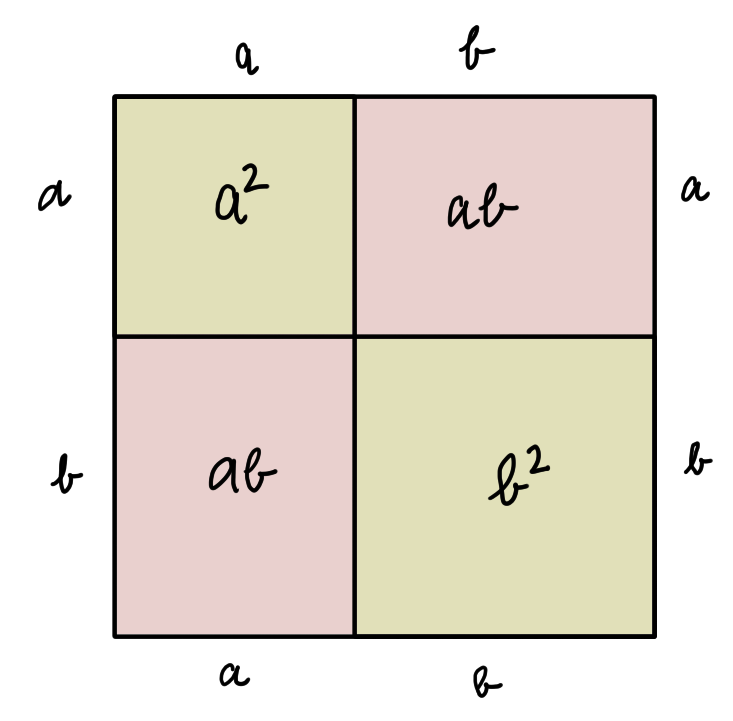
\includegraphics[width=0.5\textwidth,height=\textheight]{c02i001.png}

Or, il reste deux figures à l'extérieur des deux petits carrés. Il s'agit de deux rectangles identiques ayant pour longueur des côtés \(a\) et \(b\). L'aire de chacun est \(ab\) et l'aire des deux \(2ab\).

Nous avons réussi à exprimer l'aire totale du grand carré de deux manières différentes !

\[\text{Aire grand carré}=\text{Aire deux petits carrés} + \text{Aire deux rectangles}\]

Ce qui constitue la formule et la fin de la démonstration:

\[(a+b)^2 = a^2+2ab+b^2\]
\(\square\)

\hypertarget{bases-thuxe9oriques-1}{%
\section{Bases théoriques}\label{bases-thuxe9oriques-1}}

\hypertarget{monuxf4mes}{%
\subsection{Monômes}\label{monuxf4mes}}

\begin{defbox}
Un momôme en \(x\) est une expression de la forme
\[ax^n\qquad a\in\mathbb{Q}\text{ et } n\in\mathbb{N}\]

\end{defbox}

\hypertarget{exemples-7}{%
\subsubsection*{Exemples}\label{exemples-7}}
\addcontentsline{toc}{subsubsection}{Exemples}

\[5x^4\]
\[\dfrac{1}{3}x^3\]
\[-\dfrac{1}{3}x^2\]
\[4x\]
sont tous des \textbf{monômes en \(x\)}.

\hypertarget{remarques}{%
\subsubsection*{Remarques}\label{remarques}}
\addcontentsline{toc}{subsubsection}{Remarques}

\begin{enumerate}
\def\labelenumi{\arabic{enumi}.}
\tightlist
\item
  Tous les monômes ne sont pas des monômes en \(x\). Par exemple: \(3abc\) qui est un monôme en \(abc\); \(5a^2\) qui est un monôme en \(a\); \(4y\) qui est un monôme en \(y\).
\item
  Par convenstion, le monôme \(5\cdot a\cdot b\cdot c\) d'écrit \(5abc\).
\item
  Dans un monôme, on distingue deux parties: un coefficient et une partie littérale (voir figure).
\end{enumerate}

\hypertarget{monuxf4mes-semblables}{%
\subsubsection{Monômes semblables}\label{monuxf4mes-semblables}}

\begin{defbox}
Des monômes sont semblables si leurs parties \textbf{littérales} sont \textbf{identiques}.

\end{defbox}

\(\\[.5cm]\)

Ainsi \(5{\color{red}ab^2c}\), \(\dfrac{-1}{2}{\color{red}ab^2c}\), \(-3{\color{red}ab^2c}\) sont des monômes semblables, mais \(5ab^2c\), \(\dfrac{-1}{2}a^2bc\), \(-3a^2b^2c\) ne le sont pas.

\hypertarget{produit-de-monuxf4mes}{%
\subsubsection{Produit de monômes}\label{produit-de-monuxf4mes}}

\begin{defbox}
Il suffit de prendre des monômes et de multiplier entre elles les deux parties composant les monômes: les parties littérales entre elles et les parties numériques.

\end{defbox}

\(\\[.5cm]\)

La loi de la commutativité nous permet de commuter les facteurs au moment de la multiplication:

\begin{align*}
 -2a^3b\cdot\dfrac{3}{4}ab^2c & = \left(-2\cdot\dfrac{3}{4}\right)\cdot(a^3\cdot a)\cdot(b\cdot b^2)\cdot c\\
 & = -\dfrac{3}{2}\cdot a^4\cdot b^3\cdot c\\
 & = -\dfrac{3}{2}a^4b^3c\\
\end{align*}

\hypertarget{exemples-8}{%
\subsubsection*{Exemples}\label{exemples-8}}
\addcontentsline{toc}{subsubsection}{Exemples}

\[\dfrac{5}{3}x^3y\cdot\left(-\dfrac{2}{5}x^2\right)\cdot 3ay^2 = -2ax^5y^3\]
\[-a^2b^3\cdot\dfrac{a^3c^2}{3}\cdot\left(-\dfrac{6ab^2c}{5}\right)=\dfrac{2a^6b^5c^3}{5}\]

\hypertarget{polynuxf4mes}{%
\subsection{Polynômes}\label{polynuxf4mes}}

\begin{defbox}
Un polynôme est une \textbf{somme de monômes}.

\end{defbox}

\hypertarget{exemples-9}{%
\subsubsection*{Exemples}\label{exemples-9}}
\addcontentsline{toc}{subsubsection}{Exemples}

\[a+b\]
\[5x-3y+1\]
\[\dfrac{3}{2}a^2-\dfrac{1}{3}b^3+ ab + 5\]

sont tous des polynômes.

\hypertarget{produit-dun-polynuxf4me-par-un-monuxf4me}{%
\subsubsection{Produit d'un polynôme par un monôme}\label{produit-dun-polynuxf4me-par-un-monuxf4me}}

\hypertarget{exemples-10}{%
\paragraph*{Exemples}\label{exemples-10}}
\addcontentsline{toc}{paragraph}{Exemples}

\[3a\cdot(6b+7c) = 3a\cdot 6b+ 3a\cdot 7c = 18ab+21ac\]
\[(2x+5a)\cdot 2ax=2x\cdot 2ax + 5a\cdot 2ax = 4ax^2+10a^2x\]
\[5(a-b-c) = 5(a+(-b)+(-c))=5\cdot a+5\cdot(-b) 5\cdot(-c) = 5a-5b-5c\]

La distributivité de la multiplication par rapport à l'addition permet de multiplier le monôme par chaque terme du polynôme.

\hypertarget{la-mise-en-uxe9vidence}{%
\subsubsection*{La mise en évidence}\label{la-mise-en-uxe9vidence}}
\addcontentsline{toc}{subsubsection}{La mise en évidence}

Est une ``technique'' qui permet la factorisation. Par exemple l'égalité
\[5x(2y-z) = 10xy-5xz\]
peut être lue dans ce sens
\[10xy-5xz= 5x(2y-z)\]

Le passage de l'expression \(10xy-5xz\) à l'expression \(5x(2y-z)\) s'appelle \textbf{mise en évidence des facteurs communs} ou simplement \textbf{mise en évidence}.

En effet, dans les deux premiers termes \(10xy\) et \(5xz\) il y a un facteur commun, qui est \(5x\) justement.

Par exemple:

\begin{align*} 
16x^3y^2-24x^2y+40x^2y^2 & ={\color{red}2}\cdot {\color{red}2}\cdot {\color{red}2} \cdot 2\cdot {\color{red}x}\cdot{\color{red}x}\cdot x\cdot {\color{red}y}\cdot y - {\color{red}2}\cdot {\color{red}2}\cdot {\color{red}2} \cdot 3\cdot{\color{red}x}\cdot{\color{red}x}\cdot{\color{red}y} +{\color{red}2}\cdot {\color{red}2}\cdot {\color{red}2} \cdot 5\cdot{\color{red}x}\cdot{\color{red}x}\cdot{\color{red}y}\cdot y\\
& = {\color{red}8x^2y}(2xy-3+5y)\\
\end{align*}

\textbf{Remarquer} que le monôme \(8x^2y\) est le \textbf{PGDC} des trois termes du polynôme.

\hypertarget{somme-de-monuxf4mes-semblables}{%
\subsubsection{Somme de monômes semblables}\label{somme-de-monuxf4mes-semblables}}

\begin{defbox}
Pour effectuer la somme de \textbf{monômes semblables}, on additionne les coefficients et on garde la partie littérale.

\end{defbox}

Dans
\[5a+8a = a\cdot(5+8)=a\cdot 13=13a\]
le passage de l'expression \(5a+8a\) à l'expression \(13a\) s'appelle \textbf{réduction de termes semblables}.

\hypertarget{exemples-11}{%
\subsubsection*{Exemples}\label{exemples-11}}
\addcontentsline{toc}{subsubsection}{Exemples}

\begin{align*}
15x^2+3x^2-7x^2  & = x^2\cdot(15+3-7)=11x^2\\
\\\\
6a^2b-8a^2b-a^2b & = a^2b(6-8-1)=-3a^2b\\
\\\\
16ab+8xy-ab+2xy &= (16ab-ab)+(8xy+2xy)\\
               &= ab(16-1)+xy(8+2)\\
               &= 15ab+10xy\\
\\\\
9x^2y+12xy^2+8x^2y-5xy^2+xy-17x^2y &= 9x^2y+8x^2y-17x^2y+12xy^2-5xy^2+xy\\
&= x^2y(9+8-17)+xy^2(12-5)+xy\\
&= 7xy^2+xy\\
\end{align*}

\hypertarget{somme-et-diffuxe9rence-de-polynuxf4mes}{%
\subsubsection{Somme et différence de polynômes}\label{somme-et-diffuxe9rence-de-polynuxf4mes}}

\hypertarget{somme-de-polynuxf4mes}{%
\subsubsection*{Somme de polynômes}\label{somme-de-polynuxf4mes}}
\addcontentsline{toc}{subsubsection}{Somme de polynômes}

L'associativité de l'addition permet de supprimer les parenthèses entre les polynômes qu'on additionne:

\begin{align*}
(5x^3-8x^2-3x-4)+(-x^3+2x^2+5) & = 5x^3-8x^2-3x-4-x^3+2x^2+5\\
& = 5x^3-x^3-8x^2+2x^2-3x-4+5\\
& = 4x^3-6x^2-3x+1\\
\end{align*}

\hypertarget{diffuxe9rence-de-polynuxf4mes}{%
\subsubsection*{Différence de polynômes}\label{diffuxe9rence-de-polynuxf4mes}}
\addcontentsline{toc}{subsubsection}{Différence de polynômes}

L'opposé d'un polynôme s'obtient en changeant les signes de chacun de ses termes; il s'agit en fait d'une multiplication par \((-1)\):

\(5ax\) et \(-5ax\) sont des monômes opposés, car leur somme est nulle:
\[(5ax)+(-5ax)=0\]

\((-4x^2+3x-5)\) et \((4x^2-3x+5)\) sont des polynômes opposés, pour les mêmes raisons:
\[(-4x^2+3x-5)+(4x^2-3x+5) = -4x^2+3x-5+4x^2-3x+5=0\]

\begin{reglebox}
Pour soustraire un polynôme, on \textbf{additionne son opposé}.

\end{reglebox}

\hypertarget{exemples-12}{%
\subsubsection*{Exemples}\label{exemples-12}}
\addcontentsline{toc}{subsubsection}{Exemples}

\begin{align*}
(3a^2b-2ab+5b^2)-(4ab-3a^2b-6b^2) &= (3a^2b-2ab+5b^2)+(-4ab+3a^2b+6b^2)\\
&= 3a^2b-2ab+5b^2-4ab+3a^2b+6b^2\\
&= 6a^2b-6ab+11b^2\\
\\
(3x^2y+8xy^2)-((-xy+5xy^2)-(-11x^2y+7xy)) &=  (3x^2y+8xy^2)-((-xy+5xy^2)+(+11x^2y-7xy))\\
&=(3x^2y+8xy^2)-(-xy+5xy^2+11x^2y-7xy)\\
&=(3x^2y+8xy^2)+(+xy-5xy^2-11x^2y+7xy)\\
&=3x^2y+8xy^2+xy-5xy^2-11x^2y+7xy\\
&=-8x^2y+3xy^2+8xy\\
\\
8(a+b)-3(a-b) &=(8(a+b))-(3(a-b))\\
&=(8a+8b)-(3a-3b)\\
&=(8a+8b)+(-3a+3b)\\
&=8a+8b-3a+3b\\
&=5a+11b\\
\end{align*}

\hypertarget{produit-de-polynuxf4mes}{%
\subsubsection{Produit de polynômes}\label{produit-de-polynuxf4mes}}

Comment effectuer le produit \((a+b)\cdot (c+d)\) ?

Si on pose \((a+b)=u\), on obtient \[{\color{red}u}\cdot(c+d) = {\color{red}u}\cdot c + {\color{red}u}\cdot d\]
et donc

\[{\color{red}(a+b)}\cdot(c+d) = {\color{red}(a+b)}\cdot c + {\color{red}(a+b)}\cdot d\]

La distributivité de la multiplication par rapport à l'addition permet de multiplier chaque terme du premier polynôme par chaque terme du second.

\begin{reglebox}
\[(a+b)\cdot(c+d)=ac+ad+bc+bd\]

\end{reglebox}

\hypertarget{exemples-13}{%
\subsubsection*{Exemples}\label{exemples-13}}
\addcontentsline{toc}{subsubsection}{Exemples}

\begin{align*}
(2x-3y)\cdot(x+y) & =2x^2+2xy-3xy-3y^2\\
& = 2x^2-xy-3y^2\\
\\
(x+3)\cdot(x-5)\cdot(x+4) &= ((x+3)(x-5))\cdot(x+4)\\
&=(x^2-5x+3x-15)(x+4)\\
&=(x^2-2x-15)(x+4)\\
&=x^3+2x^2-23x-60\\
\end{align*}

\hypertarget{produits-remarquables}{%
\subsubsection{Produits remarquables}\label{produits-remarquables}}

Certains produits de polynômes se rencontrent fréquemment; on les appelle produits remarquables.

\hypertarget{carruxe9-dune-somme-de-deux-termes}{%
\subsubsection*{Carré d'une somme de deux termes}\label{carruxe9-dune-somme-de-deux-termes}}
\addcontentsline{toc}{subsubsection}{Carré d'une somme de deux termes}

L'expression \((x+y)^2\) peut être développée comme suit \[(x+y)^2=(x+y)(x+y)=x^2+xy+xy+y^2= x^2+2xy+y^2\]

Et on a

\begin{reglebox}
\[(a+b)^2 = a^2 + 2ab + b^2\]

\end{reglebox}

\hypertarget{exemples-14}{%
\subsubsection*{Exemples}\label{exemples-14}}
\addcontentsline{toc}{subsubsection}{Exemples}

\begin{align*}
23^2 &=(20+3)^2\\
    &=20^2+2\cdot 20\cdot 3+3^2 = 400+120+9=529\\
    \\
(3x+5y)^2 &= (3x)^2+2\cdot 3x \cdot 5y + (5y)^2\\
&= 9x^2+30xy+25y^2\\
\\
(\dfrac{1}{2}+2x)^2 &= (\dfrac{1}{2})^2+2\cdot\dfrac{1}{2}\cdot 2x+(2x)^2\\
&=\dfrac{1}{4}+2x+4x^2\\
\end{align*}

\hypertarget{carruxe9-dune-somme-de-deux-termes-1}{%
\subsubsection*{Carré d'une somme de deux termes}\label{carruxe9-dune-somme-de-deux-termes-1}}
\addcontentsline{toc}{subsubsection}{Carré d'une somme de deux termes}

\[(x-y)^2=(x-y)(x-y)=x^2-xy-xy+y^2=x^2-2xy+y^2\]

\begin{reglebox}
\[(a-b)^2 = a^2 - 2ab + b^2\]

\end{reglebox}

\hypertarget{exemples-15}{%
\subsubsection*{Exemples}\label{exemples-15}}
\addcontentsline{toc}{subsubsection}{Exemples}

\begin{align*}
38^2=(40-2)^2 & = 40^2-2\cdot 40\cdot 2+2^2\\
&= 1600-160+4\\
&= 1444\\
\\
(0{,}2x-1{,}2x)^2 &= (0{,}2x)^2-2\cdot 0{,}2x\cdot 1{,}2y+(1{,}2y)^2\\
&= 0{,}04x^2 - 0{,}48xy + 1{,}44y^2\\
\\
(3a^3-2a^2)^2 &= (3a^3)^2-2\cdot 3a^3\cdot 2a^2+(2a^2)^2\\
&= 9a^6 - 12a^5 + 4a^4\\
\end{align*}

\hypertarget{produit-dune-somme-de-deux-termes-par-leur-diffuxe9rence}{%
\subsubsection*{Produit d'une somme de deux termes par leur différence}\label{produit-dune-somme-de-deux-termes-par-leur-diffuxe9rence}}
\addcontentsline{toc}{subsubsection}{Produit d'une somme de deux termes par leur différence}

\[(x+y)\cdot(x-y) = x^2-xy+xy-y^2=x^2-y^2\]

\begin{reglebox}
\[(a+b)\cdot(a-b) = a^2-b^2\]

\end{reglebox}

\hypertarget{exemples-16}{%
\subsubsection*{Exemples}\label{exemples-16}}
\addcontentsline{toc}{subsubsection}{Exemples}

\begin{align*}
81\cdot 79 & = (80+1)\cdot (80-1)\\
&= 80^2 -1^2 \\
&= 6400-1\\
&= 6399\\
\\
(3a+2b)\cdot(3a-2b) &= (3a)^2-(2b)^2\\
&= 9a^2-4b^2\\
\\
(x+1)(x-1)\cdot(x^2-1) &= (x^2-1)\cdot(x^2-1)\\
&= x^4-2x^2+1\\
\end{align*}

\hypertarget{factorisation}{%
\subsubsection{Factorisation}\label{factorisation}}

\begin{defbox}
Factoriser une expression c'est la décomposer en un produit de facteurs.

\end{defbox}

\(\\[0.5cm]\)

Pour factoriser, on utilise essentiellement deux techniques:

\begin{enumerate}
\def\labelenumi{\alph{enumi}.}
\item
  \textbf{La mise en évidence}

  Par exemple: \[25a^2+15ab-5a = 5a(5a+3b-1)\] où on applique une distributivité si on lit de droite à gauche.
\item
  \textbf{Les produits remarquables}

  Par exemple:
  \begin{align*}
   4x^4 + 12x^2y+9y^2 &= (2x^2+3y)^2\\
   \\
   a^2-a+\dfrac{1}{4} &= (a-\dfrac{1}{2})^2\\
   \\
   16x^2-0{,}25 &= (4x-0{,}5)(4x+0{,}5)\\
   \\
   x^4-1 &= (x^2+1)\cdot(x^2-1)\\
         & =(x^2+1)(x-1)(x+1)\\
  \end{align*}
\end{enumerate}

\hypertarget{remarque-1}{%
\subsubsection*{Remarque}\label{remarque-1}}
\addcontentsline{toc}{subsubsection}{Remarque}

On utilise parfois les deux techniques de factorisation dans une même expression.
Par exemple:

\begin{align*}
6x^2+24x+24 &= 6(x^2+4x+4)\\
            &= 6(x+2)^2\\
\\
5a^8-5 &= 5(a^8-1)\\
       &= 5(a^4+1)(a^2+1)(a-1)(a+1)\\
\end{align*}

\hypertarget{exercices-ruxe9solus-exemples-1}{%
\section{Exercices résolus (exemples)}\label{exercices-ruxe9solus-exemples-1}}

\hypertarget{exemple-1-2}{%
\subsection{Exemple 1}\label{exemple-1-2}}

Effectuer le produit suivant \((x+a)\cdot 5\).

\hypertarget{solution-1-1}{%
\subsection*{Solution 1}\label{solution-1-1}}
\addcontentsline{toc}{subsection}{Solution 1}

On observe l'expression. Il s'agit d'une parenthèse, comportant une addition et d'un facteur (\(5\)) qui la multiplie. Seulement ce facteur est à droite de la parenthèse.

Cela ne pose aucun problème, car \((x+a)\cdot 5 = 5\cdot (x+a)\), grâce à la commutativité de la multiplication.

On doit donc distribuer le facteur \(5\) dans la parenthèse. La solution s'écrit:

\[(x+a)\cdot 5= 5x+5a\]

\hypertarget{exemple-2-2}{%
\subsection{Exemple 2}\label{exemple-2-2}}

Développer le produit suivant \((2ab-3a+b)\cdot 5x\).

\hypertarget{solution-2-1}{%
\subsection*{Solution 2}\label{solution-2-1}}
\addcontentsline{toc}{subsection}{Solution 2}

La seule différence par rapport à l'exemple précédent c'est que la parenthèse est composée de la somme de trois monômes, autrement dit un polynôme à trois termes.

La solution s'écrit donc ainsi

\begin{align*}
(2ab-3a+b)\cdot 5x & =2ab\cdot 5x-3a\cdot 5x + b\cdot 5x \\
& = 10abx-15ax+5bx
\end{align*}

\hypertarget{exemple-3}{%
\subsection{Exemple 3}\label{exemple-3}}

Factorise le polynôme suivant \[9a^2b^2-27ab+63a\]

\hypertarget{solution-3}{%
\subsection*{Solution 3}\label{solution-3}}
\addcontentsline{toc}{subsection}{Solution 3}

On se souvient que \textbf{factoriser} c'est décomposer une somme en un produit. On utilise pour ce faire une mise en évidence des facteurs ``qui se retrouvent'' dans chacun des termes du polynôme.

Ici, chaque partie numérique des termes est un multiple de \(9\) et on voit que du côté des lettres, c'est le \(a\) qui se retrouve dans tous les termes. On a donc trouvé notre facteur commun: \(9a\).

On met ce facteur \textbf{à l'extérieur d'une paire de parenthèses}. L'intérieur de la parenthèse contiendra le quotient de chaque terme par \(9a\). Autrement dit, on va diviser chacun des termes par \(9a\) et écrire le résultat dans la parenthèse:

\[9a^2b^2-27ab+63a=9a(ab^2-3b+7)\]

et nous avons transformé la somme en un produit, c'est-à-dire, nous avons factorisé l'expression de départ.

\hypertarget{exercices-et-probluxe8mes-1}{%
\section{Exercices et problèmes}\label{exercices-et-probluxe8mes-1}}

\hypertarget{exercices-i-1}{%
\subsection{Exercices (I)}\label{exercices-i-1}}

\hypertarget{exercice-1-2}{%
\subsubsection*{Exercice 1}\label{exercice-1-2}}
\addcontentsline{toc}{subsubsection}{Exercice 1}

Parmi les monômes suivants, groupe ceux qui sont semblables

\(\begin{array}{lcr} 3x^2y & 3xy^2 & -3x^2y^2\\ \dfrac{1}{2}x^2y & -\dfrac{2}{3}x^2y^2 & \dfrac{3}{5}x^3y^2\\ 2\cdot x \cdot y^2 & -\dfrac{2}{7}x\cdot y^2\cdot xy & -5y^2\cdot x\\ 4\cdot x\cdot y\cdot x\quad & -\dfrac{1}{2}y^3x^2 &\quad -0{,}2x^2\cdot y\cdot xy\\ \end{array}\)

\hypertarget{exercice-2-1}{%
\subsubsection*{Exercice 2}\label{exercice-2-1}}
\addcontentsline{toc}{subsubsection}{Exercice 2}

Calcule la valeur des monômes suivants si \(a=-1\) et \(b=2\)

\begin{enumerate}
\def\labelenumi{\arabic{enumi}.}
\tightlist
\item
  \(\quad3a^2b\)
\item
  \(\quad-2a^3b^2\)
\item
  \(\quad\dfrac{1}{2}a^3b\)
\item
  \(\quad-\dfrac{1}{3}a^2b^2\)
\item
  \(\quad\dfrac{3}{4}a^4b^3\)
\item
  \(\quad-5a^5b^4\)
\item
  \(\quad-\dfrac{1}{6}ab^3\)
\item
  \(\quad\dfrac{3}{5}a^6b^3\)
\end{enumerate}

\hypertarget{exercice-3-2}{%
\subsubsection*{Exercice 3}\label{exercice-3-2}}
\addcontentsline{toc}{subsubsection}{Exercice 3}

Effectue le produit des monômes suivants

\begin{enumerate}
\def\labelenumi{\arabic{enumi}.}
\tightlist
\item
  \(\quad 3x^2\cdot 2y \cdot 5y^3\cdot 4x^3\)
\item
  \(\quad 2a^2\cdot (-5ab)\cdot 3ab^3\)
\item
  \(\quad ay^3\cdot\left(-\dfrac{1}{2}ay^2\right)\cdot 5a^5\)
\item
  \(\quad 4b^2\cdot \dfrac{1}{2}a^3\cdot \dfrac{3}{5}a^2\)
\item
  \(\quad 5y^3\cdot(-3b^3)\cdot\frac{2}{15}b^2y\cdot a^0\)
\item
  \(\quad 2x^3y^2\cdot \left(-\dfrac{3}{4}xy^2\right)\cdot\dfrac{1}{3}x^3\)
\item
  \(\quad \dfrac{5}{8}\cdot 3a^3b^2\cdot\left(-\dfrac{2}{3}b^5\right)\cdot(-12a^3)\)
\item
  \(\quad -x\cdot (-5a^3)\cdot\left(\dfrac{-2a^2y^3}{3}\right)\cdot\left(-\dfrac{1}{7}y^2x\right)\)
\end{enumerate}

\hypertarget{exercice-4-2}{%
\subsubsection*{Exercice 4}\label{exercice-4-2}}
\addcontentsline{toc}{subsubsection}{Exercice 4}

Ecris les monômes sous leur forme réduite

\begin{enumerate}
\def\labelenumi{\arabic{enumi}.}
\tightlist
\item
  \(\quad 2(a^2x)^2\)
\item
  \(\quad -5a(x^2y)^4\)
\item
  \(\quad (-2a^2x)^2\)
\item
  \(\quad -(3x^3y^2)^4\)
\item
  \(\quad (-2a^3)^2\cdot 3a^4\)
\item
  \(\quad -(3x^3y)^2\cdot 2(xy^2)^3\)
\item
  \(\quad (-0{,}1x^2y)^3\cdot(10x^3y^2)^2\)
\item
  \(\quad \left(\dfrac{2}{3}x^2y^3\right)^2\cdot\left(-\dfrac{3}{5}xy^2\right)\)
\end{enumerate}

\hypertarget{exercice-5-2}{%
\subsubsection*{Exercice 5}\label{exercice-5-2}}
\addcontentsline{toc}{subsubsection}{Exercice 5}

Effectue les produits

\begin{enumerate}
\def\labelenumi{\arabic{enumi}.}
\tightlist
\item
  \(\quad x(x+y)\)
\item
  \(\quad a(a^2+a)\)
\item
  \(\quad 2y(a-y)\)
\item
  \(\quad (a^3-a^2)\cdot 2a\)
\item
  \(\quad (x^3+xy)\cdot x^2\)
\item
  \(\quad (-y^3)\cdot(ay-y^2)\)
\item
  \(\quad 2a^2(a-3b)\)
\item
  \(\quad 5x^2(x^3-2+z^2)\)
\item
  \(\quad (y^3+2ay+y^2)\cdot 3y^2\)
\item
  \(\quad (-4a^3)\cdot(2ab+3a^2-1)\)
\item
  \(\quad (5x^2y+2xy^2-x^3y)\cdot x^2y\)
\item
  \(\quad (-2z^2)\cdot(-5+3z-z^3)\)
\end{enumerate}

\hypertarget{exercices-ii-1}{%
\subsection{Exercices (II)}\label{exercices-ii-1}}

\hypertarget{exercice-1-3}{%
\subsubsection*{Exercice 1}\label{exercice-1-3}}
\addcontentsline{toc}{subsubsection}{Exercice 1}

Mets en évidence les facteurs communs

\begin{enumerate}
\def\labelenumi{\arabic{enumi}.}
\tightlist
\item
  \(\quad 2a+4b\)
\item
  \(\quad 5x-15y\)
\item
  \(\quad 12a+15b-9c\)
\item
  \(\quad 8x -4y +2\)
\item
  \(\quad 5a + 7ab\)
\item
  \(\quad ab+ac\)
\item
  \(\quad 2x+4xy-2xz\)
\item
  \(\quad 3a+2a\)
\item
  \(\quad xy+2x\)
\item
  \(\quad 4ac-4bc\)
\end{enumerate}

\hypertarget{exercice-2-2}{%
\subsubsection*{Exercice 2}\label{exercice-2-2}}
\addcontentsline{toc}{subsubsection}{Exercice 2}

Mets en évidence et réduis les termes semblables s'il y a lieu

\begin{enumerate}
\def\labelenumi{\arabic{enumi}.}
\tightlist
\item
  \(\quad 3a+4a\)
\item
  \(\quad 3a+6\)
\item
  \(\quad 5a-3a\)
\item
  \(\quad 4a+3\)
\item
  \(\quad 4xy+6xy\)
\item
  \(\quad 4xy+3xy-xy\)
\item
  \(\quad 2a-5a\)
\item
  \(\quad 2a-5\)
\item
  \(\quad 3ab-4ab-2ab\)
\item
  \(\quad -3x+4x\)
\item
  \(\quad -2xy-5xy+3xy\)
\item
  \(\quad 3xy+4xy-xy\)
\end{enumerate}

\hypertarget{exercice-3-3}{%
\subsubsection*{Exercice 3}\label{exercice-3-3}}
\addcontentsline{toc}{subsubsection}{Exercice 3}

Réduis les monômes semblables

\begin{enumerate}
\def\labelenumi{\arabic{enumi}.}
\tightlist
\item
  \(\quad 6x-4y-4x+7y\)
\item
  \(\quad 3c-8d-18d+5c\)
\item
  \(\quad 3{,}8u-5{,}9u+3{,}5v-3{,}5\)
\item
  \(\quad 3xy -4x^2y+5xy-x^2y\)
\item
  \(\quad 8x^2-3x^3-(-5x^2)-x^3\)
\item
  \(\quad 4x-(-2y)-(-2x)-y\)
\item
  \(\quad 2abc -3ab^2-(-abc)\)
\item
  \(\quad 18ab^2-3a^2b-8a^2b+5ab^2\)
\item
  \(\quad -(-5uv)-10u^2v+uv-(-u^2v)\)
\item
  \(\quad a-(-2b)+(-3a)-(-2a)-4b\)
\end{enumerate}

\hypertarget{exercice-4-3}{%
\subsubsection*{Exercice 4}\label{exercice-4-3}}
\addcontentsline{toc}{subsubsection}{Exercice 4}

Effectue

\begin{enumerate}
\def\labelenumi{\arabic{enumi}.}
\tightlist
\item
  \(\quad (a+b)(c-d)\)
\item
  \(\quad (a+3)(c-4)\)
\item
  \(\quad (2a+b)(c-d)\)
\item
  \(\quad (3a+b)(2c-d)\)
\item
  \(\quad (4a+b)(3c-d)\)
\item
  \(\quad (7a-3b)(4c-3d)\)
\item
  \(\quad (4c-2d)(6a+3b)\)
\item
  \(\quad (5a-b)(5b-a)\)
\end{enumerate}

\hypertarget{exercice-5-3}{%
\subsubsection*{Exercice 5}\label{exercice-5-3}}
\addcontentsline{toc}{subsubsection}{Exercice 5}

Effectue

\begin{enumerate}
\def\labelenumi{\arabic{enumi}.}
\tightlist
\item
  \(\quad 2a(3-2b)+a\)
\item
  \(\quad 3a+(5+2a)a\)
\item
  \(\quad 2x(4-2y)+x(3y-5)\)
\item
  \(\quad (-a)(2a-3)+2a^2\)
\item
  \(\quad 4x+(6-2x)(-5a)\)
\item
  \(\quad (-2c)(c-d)+(c+d)(-2c)\)
\end{enumerate}

\hypertarget{probluxe8mes-iii-1}{%
\subsection{Problèmes (III)}\label{probluxe8mes-iii-1}}

\hypertarget{probluxe8me-1-1}{%
\subsubsection*{Problème 1}\label{probluxe8me-1-1}}
\addcontentsline{toc}{subsubsection}{Problème 1}

Factorise

\begin{enumerate}
\def\labelenumi{\arabic{enumi}.}
\tightlist
\item
  \(\quad (4a+5b)(x-y)+6c(x-y)\)
\item
  \(\quad 5x(a+2b)+(y-z)(a+2b)\)
\item
  \(\quad -5a(b+c)-(b+c)\)
\item
  \(\quad b(2x+y)-(a+c)(y+2x)\)
\item
  \(\quad (2x-3a)\cdot 5b+(6b-3y)(2x-3a)\)
\item
  \(\quad (x-2y)\cdot 5x+5x(x-2y)\)
\end{enumerate}

\hypertarget{probluxe8me-2-1}{%
\subsubsection*{Problème 2}\label{probluxe8me-2-1}}
\addcontentsline{toc}{subsubsection}{Problème 2}

Factorise en utilisant si possible les produits remarquables

\begin{enumerate}
\def\labelenumi{\arabic{enumi}.}
\tightlist
\item
  \(\quad 36a^2-60ab+25b^2\)
\item
  \(\quad 4x^2-2xy+\dfrac{1}{4}y^2\)
\item
  \(\quad 9x^2-4xy+\dfrac{4}{9}y^2\)
\item
  \(\quad x^2-\dfrac{1}{2}xy+\dfrac{1}{16}y^2\)
\item
  \(\quad 4a^2-a+\dfrac{1}{16}\)
\item
  \(\quad 16y^2-24yz+4z^2\)
\end{enumerate}

\hypertarget{probluxe8me-3-1}{%
\subsubsection*{Problème 3}\label{probluxe8me-3-1}}
\addcontentsline{toc}{subsubsection}{Problème 3}

Factoriser

\begin{enumerate}
\def\labelenumi{\arabic{enumi}.}
\tightlist
\item
  \(\quad a^2-b^2\)
\item
  \(\quad y^2-z^2\)
\item
  \(\quad 4a^2-b^2\)
\item
  \(\quad 16x^2-25y^2\)
\item
  \(\quad x^4-1\)
\item
  \(\quad 25c^2-30d^2\)
\item
  \(\quad 1-16a^4\)
\item
  \(\quad 49-64x^2\)
\end{enumerate}

\hypertarget{probluxe8me-4-1}{%
\subsubsection*{Problème 4}\label{probluxe8me-4-1}}
\addcontentsline{toc}{subsubsection}{Problème 4}

Factoriser

\begin{enumerate}
\def\labelenumi{\arabic{enumi}.}
\tightlist
\item
  \(\quad 3x^2-3y^2\)
\item
  \(\quad 8a^2-16b^2\)
\item
  \(\quad 3x^2-3xy+\dfrac{3}{4}y^2\)
\item
  \(\quad \dfrac{1}{2}x^2-8\)
\item
  \(\quad 3x^2+30x+75\)
\item
  \(\quad \dfrac{1}{4}z^2-zu+u^2\)
\item
  \(\quad 0{,}08a^2-0{,}24ab+0{,}18b^2\)
\item
  \(\quad 5x^4-3125\)
\end{enumerate}

\hypertarget{probluxe8me-5}{%
\subsubsection*{Problème 5}\label{probluxe8me-5}}
\addcontentsline{toc}{subsubsection}{Problème 5}

Factoriser

\begin{enumerate}
\def\labelenumi{\arabic{enumi}.}
\tightlist
\item
  \(\quad 7ax^8-7a\)
\item
  \(\quad 16ax^2+5axy+\dfrac{25}{64}ay^2\)
\item
  \(\quad 100+20x+x^2\)
\item
  \(\quad 48-3x^2\)
\item
  \(\quad (x+y)(x^2-y^2)+(x^2-y^2)\)
\item
  \(\quad 1 - 0{,}25z^2\)
\item
  \(\quad 37x^5b^3-148x^3b^3\)
\item
  \(\quad 16a^5b+16a^4b^2+4a^3b^3\)
\item
  \(\quad (x+y)(u-v)-(u-v)\)
\item
  \(\quad -a^2+2ab-b^2\)
\end{enumerate}

\hypertarget{semaine-3-calcul-littuxe9ral-3}{%
\chapter{Semaine 3 : Calcul littéral (3)}\label{semaine-3-calcul-littuxe9ral-3}}

\hypertarget{exemple-dintroduction-2}{%
\section{Exemple d'introduction}\label{exemple-dintroduction-2}}

\hypertarget{ce-que-lalguxe8bre-peut-nous-apporter}{%
\subsection{Ce que l'algèbre peut nous apporter}\label{ce-que-lalguxe8bre-peut-nous-apporter}}

Il est commun d'entendre des gens râler au sujet des mathématiques, et de l'algèbre en particulier.

C'est par exemple le cas du célèbre essayiste français Stendhal, qui écrivait:

\emph{Suivant moi l'hypocrisie était impossible en mathématiques{[}\ldots{]} Que devins-je quand je m'aperçus que personne ne pouvrait m'expliquer comment il se faisait que : moins par moins donne plus.} (Vie de Henry Brulard)

Il y a aussi un personnage de Geoffry Willians et Ronald Searle (\textbf{Ra le bol de l'écol}, 1953) qui a une vision assez primitive de la vie et qui dit, au sujet d'un exercice d'algèbre: ``C'est juste un tas de lettres \ldots{}'', avant de lancer des injures à l'enseignant. C'est certainement que personne n'a pris la peine de lui expliquer à quoi peut nous servir l'algèbre.

Chisissez un nombre de trois chiffres.

N'importe quel nombre convient tant que la différence entre son premier et son dernier chiffre est au moins égale à deux.

Ensuite, retournez-le et soustrayez le plus petit nombre au plus grand. Ainsi, on aura par exemple

\[728-287=495\]

Enfin, retournez ce nouveau nombre à trois chiffres et additionnez-le avec le précédent:

\[495+594=1089\]

Á la fin de ce processus, on obtient \(1089\): on s'attend bien sûr à ce que ce résultat dépende du nombre à trois chiffres choisi au dépar. Mais en fait il n'en est rien: le résultat final sera toujours
\[\Huge 1089\]

Comment est-ce possible ?

L'algèbre (calcul littéral) nous montre que c'est le cas.

On a dit plus tôt dans le cours, que l'avantage de travailler avec des lettre est de considérer une infinité de nombres avec peut, une lettre. Voyons comment on peut l'expliquer.

La première étape consiste à choisir un nombre de trois chiffres, à le renverser, puis à retrancher au plus grand le plus petit.

Supposons alors que le plus grand nombre s'écrive avec trois chiffres \(a,~b\) et \(c\). Alors, en fait, il vaut
\[100a+10b+c\]

(ce qui constitue un polynôme) et après l'avoir retourné, puis avoir effectué la soustraction, on obtient \[100a + 10b +c - (100c + 10b + a)\]

Dans cette expression \(100c + 10b + a\), est le nombre choisi retourné. Si nous effectuons la soustraction des deux polynômes, on a

\begin{align*}
100a + 10b +c - (100c + 10b + a) &= 100a -100c +10b -10b +c -a\\
                                 &= 100a - a - 100c -c\\
                                 &= 99a-99c\\
                                 &= 99(a-c)\\
\end{align*}

Et comme \(a\) et \(c\) sont entiers (c'est les chiffres du nombre), ce calcul montre que la première partie du tour \emph{donnera toujours un multiple de \(99\)}.

De plus, avec un petit effort de calcul, les multiples de \(99\) qui ont \(3\) chiffres sont \(198, ~297,~ 396, ~495, ~594, ~693, ~792, ~891\), et on voit immédiatement que si l'on additionne leur premier et troisième chiffres, on tombe toujours sur \(9\).

Ainsi, quand on en vient à la dernière partie du tour, qui consiste à renverser ce nombre et à l'ajouter au précédent, on obtient \(9\) paquets de \(100\) pour les chiffres des centaines, \(9\) paquets de \(1\) pour les unités, et \(2\) paquets de \(90\) pour les dizaines ce qui donne

\[\huge 900+9+180=1089\]

Et on conclut par un petit CQFD.

\hypertarget{bases-thuxe9oriques-2}{%
\section{Bases théoriques}\label{bases-thuxe9oriques-2}}

\hypertarget{comment-effectuer-un-calcul-littuxe9ral}{%
\subsection{Comment effectuer un calcul littéral}\label{comment-effectuer-un-calcul-littuxe9ral}}

On commence par bien recopier l'énoncé. Tous les signes sont importants et pouvoir se relire est aussi important que d'écrire correctement un énoncé.

Puis on agit par étapes. À chacune d'entre elles, une règle doit être appliquée, celle qui nous permets de passer à l'étape suivante.

\hypertarget{marquer-et-suxe9parer}{%
\subsection{Marquer et séparer}\label{marquer-et-suxe9parer}}

Il est utile, dans les longues expressions, de ``marquer'' les monômes semblables, ceux qu'on a déjà traité ou ceux que l'on veut marquer comme utilisés.

Ici on utilise une propriété de la multiplication bien utile et utilisée par tout mathématicien qui se respecte: la commutativité. En effet
\[A\cdot B\]
est égal à \[B\cdot A\]

et au sein d'une expression cela donnerai, par exemple

\[A\cdot(2x-3)\cdot B = A\cdot B\cdot(2x-3) = B\cdot A(2x-3)\]

\hypertarget{la-puissance-dune-parenthuxe8se}{%
\subsection{La puissance d'une parenthèse}\label{la-puissance-dune-parenthuxe8se}}

Il n'est rare de voir les élèves écrire que le carré d'une somme est égale à la somme des carrés : \((x + y)^2 = x^2 + y^2\), mais ceci est \textbf{faux}.

Soit on utilise ce qu'on appelle ``identités remarquables'' soit on applique la définition de la puissance.

Dans l'exemple la somme \(x+y\) est en fait multipliée par elle-même, ce qui, après l'avoir écrit, ouvre la possibilité de faire une double distributivité:

\begin{align*}
(x+y)^2 & =(x+y)\cdot(x+y)\\
        & =x\cdot(x+y)+y\cdot(x+y)\\
        & =x^2+xy+yx+y^2=x^2+2xy+y^2\\
\end{align*}

On applique cette propriété aussi à des puissances plus élèvées, le calcul est alors un peu long, mais rien de compliqué:

\begin{align*}
(a+b)^3 & =(a+b)\cdot(a+b)\cdot(a+b)\\
        & =(a\cdot(a+b)+b\cdot(a+b))\cdot(a+b)\\
        & =(a^2+ab+ba+b^2)\cdot(a+b)\\
        & =(a^2+2ab+b^2)\cdot(a+b)\\
        & =(a^3+2a^2b+ab^2)+(a^2b+2ab^2+b^3)\\
        & =a^3+2a^2b+ab^2+a^2b+2ab^2+b^3\\
        & =a^3+3a^2b+3ab^2+b^3\\
\end{align*}

\hypertarget{exercices-ruxe9solus-exemples-2}{%
\section{Exercices résolus (exemples)}\label{exercices-ruxe9solus-exemples-2}}

\hypertarget{exemple-1-3}{%
\subsection{Exemple 1}\label{exemple-1-3}}

Calculer, sans l'aide d'une calculatrice, le carré de \(105\). Autrement dit \[105^2\]

\hypertarget{solution-1-2}{%
\subsection*{Solution 1}\label{solution-1-2}}
\addcontentsline{toc}{subsection}{Solution 1}

On observe.

Nous constatons que l'algèbre nous est utile: pour calculer le carré d'un grand nombre, nous allons faire plusieurs calculs de nombres plus petits.

Écrivons \(105=100+5\), et calculons le carré de \(105\):

\begin{align*}
105^2 & = (100+5)^2\\
      & = 100^2 + 2\cdot 100\cdot 5 + 5^2\\
      & = 10'000 + 1'000 + 25\\
      & = 11'025\\
\end{align*}

Le résultat est donc \(11'025\).

\hypertarget{exemple-2-3}{%
\subsection{Exemple 2}\label{exemple-2-3}}

Soit la formule suivante \[A=(2a-x)^2-(a+x)^2\]
On vous demande d'isoler la variable \(x\) en vous servant du calcul littéral.

\hypertarget{solution-2-2}{%
\subsection*{Solution 2}\label{solution-2-2}}
\addcontentsline{toc}{subsection}{Solution 2}

On observe.

Nous constatons que ce n'est pas facile à première vue. Dans ce cas, nous devons commencer par faire ce que nous savons faire: modifier l'expression de droite de l'égalité.

Ce qui est remarquable dans cette expression est la différence de deux carrés. ``Bin voilà!''. C'est la clef.

Nous allons modifier le membre de droite : nous savons que \(m^2 - n^2=(m+n)\cdot(m-n)\). Donc,

\begin{align*}
 A & =(2a-x+a+x)\cdot(2a-x-a-x)\\
   & = 3a(a-x)\\
   \\
   \Longrightarrow A &= 3a\cdot(a-x)\\
\end{align*}

Or notre ``cible'' (\(x\)) est dans une parenthèse, nous ne pouvons pas l'isoler facilement. Il faut commencer par ``dégager'' le facteur de la parenthèse, car c'est ce qui accessible. Ce \(3a\) peut être manipulé.

Nous allons donc diviser des deux côtés de l'expression par \(3a\):

\[\dfrac{A}{3a}=a-x\]

Puis nous allons soustraire \(\dfrac{A}{3a}\) des deux côtés:

\[0=a-x-\dfrac{A}{3a}\]

Et enfin nous allons additionner \(x\) des deux côtés:

\[x=a-\dfrac{A}{3a}\]

C'est le résultat.

\hypertarget{exercices-et-probluxe8mes-2}{%
\section{Exercices et problèmes}\label{exercices-et-probluxe8mes-2}}

\hypertarget{exercices-i-2}{%
\subsection{Exercices (I)}\label{exercices-i-2}}

\hypertarget{exercice-1-4}{%
\subsubsection*{Exercice 1}\label{exercice-1-4}}
\addcontentsline{toc}{subsubsection}{Exercice 1}

Trouver deux nombres dont

\begin{enumerate}
\def\labelenumi{\arabic{enumi}.}
\tightlist
\item
  \(\quad\)le produit vaut \(7\) et la somme vaut \(8\)
\item
  \(\quad\)le produit vaut \(-20\) et la somme vaut \(-8\)
\item
  \(\quad\)le produit vaut \(-20\) et la somme vaut \(1\)
\item
  \(\quad\)le produit vaut \(36\) et la somme vaut \(12\)
\item
  \(\quad\)le produit vaut \(-40\) et la somme vaut \(3\)
\item
  \(\quad\)le produit vaut \(28\) et la somme vaut \(-11\)
\end{enumerate}

\hypertarget{exercice-2-3}{%
\subsubsection*{Exercice 2}\label{exercice-2-3}}
\addcontentsline{toc}{subsubsection}{Exercice 2}

Trouver deux nombres dont

\begin{enumerate}
\def\labelenumi{\arabic{enumi}.}
\tightlist
\item
  \(\quad\)le produit vaut \(10\) et la somme vaut \(-7\)
\item
  \(\quad\)le produit vaut \(-9\) et la somme vaut \(8\)
\item
  \(\quad\)le produit vaut \(-8\) et la somme vaut \(-2\)
\item
  \(\quad\)le produit vaut \(15\) et la somme vaut \(-8\)
\item
  \(\quad\)le produit vaut \(48\) et la somme vaut \(14\)
\item
  \(\quad\)le produit vaut \(24\) et la somme vaut \(11\)
\end{enumerate}

\hypertarget{exercice-3-4}{%
\subsubsection*{Exercice 3}\label{exercice-3-4}}
\addcontentsline{toc}{subsubsection}{Exercice 3}

Factoriser à l'aide des produits remarquables

\begin{enumerate}
\def\labelenumi{\arabic{enumi}.}
\tightlist
\item
  \(\quad x^2+4x-21\)
\item
  \(\quad \dfrac{1}{4}a^2+16b^2+4ab\)
\item
  \(\quad x^2+4\)
\item
  \(\quad 9a^2+6ab+b^2\)
\item
  \(\quad 9x^8-49y^2\)
\item
  \(\quad \dfrac{1}{49}a^6-\dfrac{2}{7}a^3b+b^2\)
\end{enumerate}

\hypertarget{exercice-4-4}{%
\subsubsection*{Exercice 4}\label{exercice-4-4}}
\addcontentsline{toc}{subsubsection}{Exercice 4}

Factoriser à l'aide des produits remarquables

\begin{enumerate}
\def\labelenumi{\arabic{enumi}.}
\tightlist
\item
  \(\quad 9a^4-16b^2\)
\item
  \(\quad x^2 + x -20\)
\item
  \(\quad \dfrac{1}{4}a^2+2ab+4b^2\)
\item
  \(\quad 9a^2-4b^2\)
\item
  \(\quad 0{,}01x^2-0{,}6xy+9y^2\)
\item
  \(\quad x^2+6x-16\)
\end{enumerate}

\hypertarget{exercice-5-4}{%
\subsubsection*{Exercice 5}\label{exercice-5-4}}
\addcontentsline{toc}{subsubsection}{Exercice 5}

Factoriser aussi complétement que possible

\begin{enumerate}
\def\labelenumi{\arabic{enumi}.}
\tightlist
\item
  \(\quad 4a^2+8ab+4b^2\)
\item
  \(\quad 16a^2-8ab+b^2\)
\item
  \(\quad \dfrac{1}{4}a^2+ac+c^2\)
\item
  \(\quad 5x^2+10xy+5y^2\)
\item
  \(\quad 4a^2-16ab^3+16b^6\)
\item
  \(\quad 49a^2+42ab+9b^2\)
\end{enumerate}

\hypertarget{exercices-ii-2}{%
\subsection{Exercices (II)}\label{exercices-ii-2}}

\hypertarget{exercice-1-5}{%
\subsubsection*{Exercice 1}\label{exercice-1-5}}
\addcontentsline{toc}{subsubsection}{Exercice 1}

Réduire les expressions suivantes

\begin{enumerate}
\def\labelenumi{\arabic{enumi}.}
\tightlist
\item
  \(\quad \dfrac{4}{3}x^3y^3\cdot(-3xy^3)^2\)
\item
  \(\quad 2a-(3b-(-5+3a)-4)-2a\)
\item
  \(\quad (2x^3-3y)\cdot(-3x^3+y)\)
\item
  \(\quad x+\dfrac{y}{x}\cdot(-3x^2+4xy)\)
\item
  \(\quad (2x-3y)\cdot(3x-y)-(2x-y)\cdot(5x+y)\)
\item
  \(\quad 4x-y\cdot(x-2)+3x\cdot(5+y)\)
\end{enumerate}

\hypertarget{exercice-2-4}{%
\subsubsection*{Exercice 2}\label{exercice-2-4}}
\addcontentsline{toc}{subsubsection}{Exercice 2}

Réduire les expressions suivantes

\begin{enumerate}
\def\labelenumi{\arabic{enumi}.}
\tightlist
\item
  \(\quad \dfrac{2}{3}z^2-(3z-(\dfrac{1}{3}z-\dfrac{2}{3})\cdot z+ z^2)\)
\item
  \(\quad (2x^2z)^2-(2x^3-1)\cdot(3xz^2-x^4z^2)\)
\item
  \(\quad (2a-b)\cdot a-ba\)
\item
  \(\quad 2a-b\cdot a - ba\)
\item
  \(\quad \dfrac{3x-3}{2}-\dfrac{x+2}{3}\)
\item
  \(\quad \dfrac{3}{14}\cdot\sqrt{x}\cdot\dfrac{7}{9}\cdot\sqrt{x}\)
\end{enumerate}

\hypertarget{exercice-3-5}{%
\subsubsection*{Exercice 3}\label{exercice-3-5}}
\addcontentsline{toc}{subsubsection}{Exercice 3}

Réduire

\begin{enumerate}
\def\labelenumi{\arabic{enumi}.}
\tightlist
\item
  \(\quad\dfrac{2\cdot(2a-b)}{3}-\dfrac{3\cdot(5a-2b)}{5}\)
\item
  \(\quad\left(-\dfrac{a^4b^2c^0}{4}\right)^2\)
\item
  \(\quad \dfrac{1}{2}c^2-(3c-(\dfrac{1}{2}c+3)\cdot c)\)
\item
  \(\quad (x-3)\cdot(x-3)\cdot(x+3)\)
\item
  \(\quad x^2-(x-1)\cdot(2x+1)\)
\item
  \(\quad \dfrac{3}{2}x^2y\cdot\left(\dfrac{4}{5}xy^4-\dfrac{10}{21}x^3y^2\right)\)
\end{enumerate}

\hypertarget{exercice-4-5}{%
\subsubsection*{Exercice 4}\label{exercice-4-5}}
\addcontentsline{toc}{subsubsection}{Exercice 4}

Écrire aussi simplement que possible

\begin{enumerate}
\def\labelenumi{\arabic{enumi}.}
\tightlist
\item
  \(\quad (b^2+b^2+b\cdot b\cdot b+b\cdot b)^2\)
\item
  \(\quad (2a^2-7a^2)\div(\dfrac{1}{2}a-a)\)
\item
  \(\quad \dfrac{a-2}{a^2-4x^2}\div\dfrac{1}{2x-a}\)
\item
  \(\quad (2x-3)\cdot(x+1)-(x-4)^2\)
\item
  \(\quad 3x-2y-1-(2x-y+1)\)
\item
  \(\quad \dfrac{2x-2}{x^2-6x+5}\cdot\dfrac{x-5}{4x}\)
\end{enumerate}

\hypertarget{exercice-5-5}{%
\subsubsection*{Exercice 5}\label{exercice-5-5}}
\addcontentsline{toc}{subsubsection}{Exercice 5}

Écrire aussi simplement que possible

\begin{enumerate}
\def\labelenumi{\arabic{enumi}.}
\tightlist
\item
  \(\quad \dfrac{x-2}{2}-\dfrac{3x-4}{4}\)
\item
  \(\quad \left(\dfrac{1}{2}ab^2\right)\cdot (6x^2+\dfrac{1}{2}a)^2\)
\item
  \(\quad (2x-1)^2\cdot(2x+x)^3\)
\item
  \(\quad \dfrac{1}{3}\cdot (2x-5)+\dfrac{1}{5}+\dfrac{1}{5}\cdot(-2x+1)-\dfrac{1}{9}\cdot(4x-6)\)
\item
  \(\quad \dfrac{x^2-10x+9}{x^2-18x+81}\div\dfrac{3x-3}{x^2-81}\)
\item
  \(\quad \dfrac{x^2+2x}{x^2-1}\cdot\dfrac{x^2+2x+1}{x^3+2x^2}\)
\end{enumerate}

\hypertarget{probluxe8mes-iii-2}{%
\subsection{Problèmes (III)}\label{probluxe8mes-iii-2}}

\hypertarget{probluxe8me-1-2}{%
\subsubsection*{Problème 1}\label{probluxe8me-1-2}}
\addcontentsline{toc}{subsubsection}{Problème 1}

Quel polynôme faut-il additionner à

\begin{enumerate}
\def\labelenumi{\arabic{enumi}.}
\tightlist
\item
  \(\quad -10x\) pour obtenir \(20x\) ?
\item
  \(\quad 12x\) pour obtenir \(15x+2\) ?
\item
  \(\quad 3x^2+2x-5\) pour obtenir \(8x^2-5x+2\) ?
\item
  \(\quad 2xy\) pour obtenir \(x^2+y^2\) ?
\item
  \(\quad x+1\) pour obtenir \(x-1\) ?
\item
  \(\quad 9x^2+3z^2\) pour obtenir \(y^3\) ?
\item
  \(\quad -2x^3+x^2\) pour obtenir \(-3x^3\) ?
\end{enumerate}

\hypertarget{probluxe8me-2-2}{%
\subsubsection*{Problème 2}\label{probluxe8me-2-2}}
\addcontentsline{toc}{subsubsection}{Problème 2}

Calculer (mentalement) à l'aide d'une formule

\begin{enumerate}
\def\labelenumi{\arabic{enumi}.}
\tightlist
\item
  \(\quad 32^2\)
\item
  \(\quad 73^2\)
\item
  \(\quad 101^2\)
\item
  \(\quad 1001^2\)
\item
  \(\quad 99^2\)
\item
  \(\quad 19^2\)
\item
  \(\quad 28^2\)
\item
  \(\quad 86^2\)
\item
  \(\quad 18\cdot 22\)
\item
  \(\quad 65\cdot 75\)
\item
  \(\quad 31\cdot 49\)
\item
  \(\quad 1013\cdot 987\)
\end{enumerate}

\hypertarget{probluxe8me-3-2}{%
\subsubsection*{Problème 3}\label{probluxe8me-3-2}}
\addcontentsline{toc}{subsubsection}{Problème 3}

Vérifier que l'égalité
\[x^{10}-1=(x-1)(x^9 + x^8 + x^7 + x^6 + x^5 + x^4 + x^3 + x^2 + x + 1)\]

est vraie. Ensuite

\begin{enumerate}
\def\labelenumi{\alph{enumi}.}
\tightlist
\item
  \(\quad\)en déduire que \[11^{10}-1\] est divisible par \(100\).
\item
  \(\quad\)en déduire un moyen rapide de calculer \(\alpha = 1 + 2 + 2^2 + 2^3 + 2^4 + 2^5 + 2^6 + 2^7 + 2^8 + 2^9\)
\end{enumerate}

\hypertarget{probluxe8me-4-2}{%
\subsubsection*{Problème 4}\label{probluxe8me-4-2}}
\addcontentsline{toc}{subsubsection}{Problème 4}

Une tour du jeu d'échecs placée en case \(a1\) doit se rendre à la case \(h8\), en se déplaçant horizontalement vers la droite ou verticalement vers le haut.

De combien de manières peut-elle effectuer ce déplacement ?

\hypertarget{probluxe8me-5-1}{%
\subsubsection*{Problème 5}\label{probluxe8me-5-1}}
\addcontentsline{toc}{subsubsection}{Problème 5}

\[x^4+2x^3+3x^2+2x+1\] est le carré d'un polynôme qu'il s'agit de déterminer.

\hypertarget{semaine-4-uxe9quations-linuxe9aires-1}{%
\chapter{Semaine 4 : Équations linéaires (1)}\label{semaine-4-uxe9quations-linuxe9aires-1}}

\hypertarget{exemple-dintroduction-3}{%
\section{Exemple d'introduction}\label{exemple-dintroduction-3}}

\hypertarget{bases-thuxe9oriques-3}{%
\section{Bases théoriques}\label{bases-thuxe9oriques-3}}

\hypertarget{exercices-ruxe9solus-exemples-3}{%
\section{Exercices résolus (exemples)}\label{exercices-ruxe9solus-exemples-3}}

\hypertarget{exercices-et-probluxe8mes-3}{%
\section{Exercices et problèmes}\label{exercices-et-probluxe8mes-3}}

\hypertarget{exercices-i-3}{%
\subsection{Exercices (I)}\label{exercices-i-3}}

\hypertarget{exercices-ii-3}{%
\subsection{Exercices (II)}\label{exercices-ii-3}}

\hypertarget{probluxe8mes-iii-3}{%
\subsection{Problèmes (III)}\label{probluxe8mes-iii-3}}

\hypertarget{semaine-5-uxe9quations-linuxe9aires-2}{%
\chapter{Semaine 5 : Équations linéaires (2)}\label{semaine-5-uxe9quations-linuxe9aires-2}}

\hypertarget{exemple-dintroduction-4}{%
\section{Exemple d'introduction}\label{exemple-dintroduction-4}}

\hypertarget{bases-thuxe9oriques-4}{%
\section{Bases théoriques}\label{bases-thuxe9oriques-4}}

\hypertarget{exercices-ruxe9solus-exemples-4}{%
\section{Exercices résolus (exemples)}\label{exercices-ruxe9solus-exemples-4}}

\hypertarget{exercices-et-probluxe8mes-4}{%
\section{Exercices et problèmes}\label{exercices-et-probluxe8mes-4}}

\hypertarget{exercices-i-4}{%
\subsection{Exercices (I)}\label{exercices-i-4}}

\hypertarget{exercices-ii-4}{%
\subsection{Exercices (II)}\label{exercices-ii-4}}

\hypertarget{probluxe8mes-iii-4}{%
\subsection{Problèmes (III)}\label{probluxe8mes-iii-4}}

\hypertarget{semaine-6-uxe9quations-linuxe9aires-3}{%
\chapter{Semaine 6 : Équations linéaires (3)}\label{semaine-6-uxe9quations-linuxe9aires-3}}

\hypertarget{exemple-dintroduction-5}{%
\section{Exemple d'introduction}\label{exemple-dintroduction-5}}

\hypertarget{bases-thuxe9oriques-5}{%
\section{Bases théoriques}\label{bases-thuxe9oriques-5}}

\hypertarget{exercices-ruxe9solus-exemples-5}{%
\section{Exercices résolus (exemples)}\label{exercices-ruxe9solus-exemples-5}}

\hypertarget{exercices-et-probluxe8mes-5}{%
\section{Exercices et problèmes}\label{exercices-et-probluxe8mes-5}}

\hypertarget{exercices-i-5}{%
\subsection{Exercices (I)}\label{exercices-i-5}}

\hypertarget{exercices-ii-5}{%
\subsection{Exercices (II)}\label{exercices-ii-5}}

\hypertarget{probluxe8mes-iii-5}{%
\subsection{Problèmes (III)}\label{probluxe8mes-iii-5}}

\hypertarget{semaine-7-uxe9quations-linuxe9aires-4}{%
\chapter{Semaine 7 : Équations linéaires (4)}\label{semaine-7-uxe9quations-linuxe9aires-4}}

\hypertarget{exemple-dintroduction-6}{%
\section{Exemple d'introduction}\label{exemple-dintroduction-6}}

\hypertarget{bases-thuxe9oriques-6}{%
\section{Bases théoriques}\label{bases-thuxe9oriques-6}}

\hypertarget{exercices-ruxe9solus-exemples-6}{%
\section{Exercices résolus (exemples)}\label{exercices-ruxe9solus-exemples-6}}

\hypertarget{exercices-et-probluxe8mes-6}{%
\section{Exercices et problèmes}\label{exercices-et-probluxe8mes-6}}

\hypertarget{exercices-i-6}{%
\subsection{Exercices (I)}\label{exercices-i-6}}

\hypertarget{exercices-ii-6}{%
\subsection{Exercices (II)}\label{exercices-ii-6}}

\hypertarget{probluxe8mes-iii-6}{%
\subsection{Problèmes (III)}\label{probluxe8mes-iii-6}}

\hypertarget{semaine-8-uxe9quations-linuxe9aires-5}{%
\chapter{Semaine 8 : Équations linéaires (5)}\label{semaine-8-uxe9quations-linuxe9aires-5}}

\hypertarget{exemple-dintroduction-7}{%
\section{Exemple d'introduction}\label{exemple-dintroduction-7}}

\hypertarget{bases-thuxe9oriques-7}{%
\section{Bases théoriques}\label{bases-thuxe9oriques-7}}

\hypertarget{exercices-ruxe9solus-exemples-7}{%
\section{Exercices résolus (exemples)}\label{exercices-ruxe9solus-exemples-7}}

\hypertarget{exercices-et-probluxe8mes-7}{%
\section{Exercices et problèmes}\label{exercices-et-probluxe8mes-7}}

\hypertarget{exercices-i-7}{%
\subsection{Exercices (I)}\label{exercices-i-7}}

\hypertarget{exercices-ii-7}{%
\subsection{Exercices (II)}\label{exercices-ii-7}}

\hypertarget{probluxe8mes-iii-7}{%
\subsection{Problèmes (III)}\label{probluxe8mes-iii-7}}

\hypertarget{semaine-9-systuxe8mes-linuxe9aires-1}{%
\chapter{Semaine 9 : Systèmes linéaires (1)}\label{semaine-9-systuxe8mes-linuxe9aires-1}}

\hypertarget{exemple-dintroduction-8}{%
\section{Exemple d'introduction}\label{exemple-dintroduction-8}}

\hypertarget{bases-thuxe9oriques-8}{%
\section{Bases théoriques}\label{bases-thuxe9oriques-8}}

\hypertarget{exercices-ruxe9solus-exemples-8}{%
\section{Exercices résolus (exemples)}\label{exercices-ruxe9solus-exemples-8}}

\hypertarget{exercices-et-probluxe8mes-8}{%
\section{Exercices et problèmes}\label{exercices-et-probluxe8mes-8}}

\hypertarget{exercices-i-8}{%
\subsection{Exercices (I)}\label{exercices-i-8}}

\hypertarget{exercices-ii-8}{%
\subsection{Exercices (II)}\label{exercices-ii-8}}

\hypertarget{probluxe8mes-iii-8}{%
\subsection{Problèmes (III)}\label{probluxe8mes-iii-8}}

\hypertarget{semaine-10-systuxe8mes-linuxe9aires-2}{%
\chapter{Semaine 10 : Systèmes linéaires (2)}\label{semaine-10-systuxe8mes-linuxe9aires-2}}

\hypertarget{exemple-dintroduction-9}{%
\section{Exemple d'introduction}\label{exemple-dintroduction-9}}

\hypertarget{bases-thuxe9oriques-9}{%
\section{Bases théoriques}\label{bases-thuxe9oriques-9}}

\hypertarget{exercices-ruxe9solus-exemples-9}{%
\section{Exercices résolus (exemples)}\label{exercices-ruxe9solus-exemples-9}}

\hypertarget{exercices-et-probluxe8mes-9}{%
\section{Exercices et problèmes}\label{exercices-et-probluxe8mes-9}}

\hypertarget{exercices-i-9}{%
\subsection{Exercices (I)}\label{exercices-i-9}}

\hypertarget{exercices-ii-9}{%
\subsection{Exercices (II)}\label{exercices-ii-9}}

\hypertarget{probluxe8mes-iii-9}{%
\subsection{Problèmes (III)}\label{probluxe8mes-iii-9}}

\hypertarget{semaine-11-systuxe8mes-linuxe9aires-3}{%
\chapter{Semaine 11 : Systèmes linéaires (3)}\label{semaine-11-systuxe8mes-linuxe9aires-3}}

\hypertarget{exemple-dintroduction-10}{%
\section{Exemple d'introduction}\label{exemple-dintroduction-10}}

\hypertarget{bases-thuxe9oriques-10}{%
\section{Bases théoriques}\label{bases-thuxe9oriques-10}}

\hypertarget{exercices-ruxe9solus-exemples-10}{%
\section{Exercices résolus (exemples)}\label{exercices-ruxe9solus-exemples-10}}

\hypertarget{exercices-et-probluxe8mes-10}{%
\section{Exercices et problèmes}\label{exercices-et-probluxe8mes-10}}

\hypertarget{exercices-i-10}{%
\subsection{Exercices (I)}\label{exercices-i-10}}

\hypertarget{exercices-ii-10}{%
\subsection{Exercices (II)}\label{exercices-ii-10}}

\hypertarget{probluxe8mes-iii-10}{%
\subsection{Problèmes (III)}\label{probluxe8mes-iii-10}}

\hypertarget{semaine-12-inuxe9quations-linuxe9aires-1}{%
\chapter{Semaine 12 : Inéquations linéaires (1)}\label{semaine-12-inuxe9quations-linuxe9aires-1}}

\hypertarget{exemple-dintroduction-11}{%
\section{Exemple d'introduction}\label{exemple-dintroduction-11}}

\hypertarget{bases-thuxe9oriques-11}{%
\section{Bases théoriques}\label{bases-thuxe9oriques-11}}

\hypertarget{exercices-ruxe9solus-exemples-11}{%
\section{Exercices résolus (exemples)}\label{exercices-ruxe9solus-exemples-11}}

\hypertarget{exercices-et-probluxe8mes-11}{%
\section{Exercices et problèmes}\label{exercices-et-probluxe8mes-11}}

\hypertarget{exercices-i-11}{%
\subsection{Exercices (I)}\label{exercices-i-11}}

\hypertarget{exercices-ii-11}{%
\subsection{Exercices (II)}\label{exercices-ii-11}}

\hypertarget{probluxe8mes-iii-11}{%
\subsection{Problèmes (III)}\label{probluxe8mes-iii-11}}

\hypertarget{semaine-13-inuxe9quations-linuxe9aires-2}{%
\chapter{Semaine 13 : Inéquations linéaires (2)}\label{semaine-13-inuxe9quations-linuxe9aires-2}}

\hypertarget{exemple-dintroduction-12}{%
\section{Exemple d'introduction}\label{exemple-dintroduction-12}}

\hypertarget{bases-thuxe9oriques-12}{%
\section{Bases théoriques}\label{bases-thuxe9oriques-12}}

\hypertarget{exercices-ruxe9solus-exemples-12}{%
\section{Exercices résolus (exemples)}\label{exercices-ruxe9solus-exemples-12}}

\hypertarget{exercices-et-probluxe8mes-12}{%
\section{Exercices et problèmes}\label{exercices-et-probluxe8mes-12}}

\hypertarget{exercices-i-12}{%
\subsection{Exercices (I)}\label{exercices-i-12}}

\hypertarget{exercices-ii-12}{%
\subsection{Exercices (II)}\label{exercices-ii-12}}

\hypertarget{probluxe8mes-iii-12}{%
\subsection{Problèmes (III)}\label{probluxe8mes-iii-12}}

\hypertarget{semaine-14-inuxe9quations-linuxe9aires-3}{%
\chapter{Semaine 14 : Inéquations linéaires (3)}\label{semaine-14-inuxe9quations-linuxe9aires-3}}

\hypertarget{exemple-dintroduction-13}{%
\section{Exemple d'introduction}\label{exemple-dintroduction-13}}

\hypertarget{bases-thuxe9oriques-13}{%
\section{Bases théoriques}\label{bases-thuxe9oriques-13}}

\hypertarget{exercices-ruxe9solus-exemples-13}{%
\section{Exercices résolus (exemples)}\label{exercices-ruxe9solus-exemples-13}}

\hypertarget{exercices-et-probluxe8mes-13}{%
\section{Exercices et problèmes}\label{exercices-et-probluxe8mes-13}}

\hypertarget{exercices-i-13}{%
\subsection{Exercices (I)}\label{exercices-i-13}}

\hypertarget{exercices-ii-13}{%
\subsection{Exercices (II)}\label{exercices-ii-13}}

\hypertarget{probluxe8mes-iii-13}{%
\subsection{Problèmes (III)}\label{probluxe8mes-iii-13}}

\hypertarget{semaine-15-proportionnalituxe9-1}{%
\chapter{Semaine 15 : Proportionnalité (1)}\label{semaine-15-proportionnalituxe9-1}}

\hypertarget{exemple-dintroduction-14}{%
\section{Exemple d'introduction}\label{exemple-dintroduction-14}}

\hypertarget{bases-thuxe9oriques-14}{%
\section{Bases théoriques}\label{bases-thuxe9oriques-14}}

\hypertarget{exercices-ruxe9solus-exemples-14}{%
\section{Exercices résolus (exemples)}\label{exercices-ruxe9solus-exemples-14}}

\hypertarget{exercices-et-probluxe8mes-14}{%
\section{Exercices et problèmes}\label{exercices-et-probluxe8mes-14}}

\hypertarget{exercices-i-14}{%
\subsection{Exercices (I)}\label{exercices-i-14}}

\hypertarget{exercices-ii-14}{%
\subsection{Exercices (II)}\label{exercices-ii-14}}

\hypertarget{probluxe8mes-iii-14}{%
\subsection{Problèmes (III)}\label{probluxe8mes-iii-14}}

\hypertarget{semaine-16-proportionnalituxe9-2}{%
\chapter{Semaine 16 : Proportionnalité (2)}\label{semaine-16-proportionnalituxe9-2}}

\hypertarget{exemple-dintroduction-15}{%
\section{Exemple d'introduction}\label{exemple-dintroduction-15}}

\hypertarget{bases-thuxe9oriques-15}{%
\section{Bases théoriques}\label{bases-thuxe9oriques-15}}

\hypertarget{exercices-ruxe9solus-exemples-15}{%
\section{Exercices résolus (exemples)}\label{exercices-ruxe9solus-exemples-15}}

\hypertarget{exercices-et-probluxe8mes-15}{%
\section{Exercices et problèmes}\label{exercices-et-probluxe8mes-15}}

\hypertarget{exercices-i-15}{%
\subsection{Exercices (I)}\label{exercices-i-15}}

\hypertarget{exercices-ii-15}{%
\subsection{Exercices (II)}\label{exercices-ii-15}}

\hypertarget{probluxe8mes-iii-15}{%
\subsection{Problèmes (III)}\label{probluxe8mes-iii-15}}

\hypertarget{semaine-17-proportionnalituxe9-3}{%
\chapter{Semaine 17 : Proportionnalité (3)}\label{semaine-17-proportionnalituxe9-3}}

\hypertarget{exemple-dintroduction-16}{%
\section{Exemple d'introduction}\label{exemple-dintroduction-16}}

\hypertarget{bases-thuxe9oriques-16}{%
\section{Bases théoriques}\label{bases-thuxe9oriques-16}}

\hypertarget{exercices-ruxe9solus-exemples-16}{%
\section{Exercices résolus (exemples)}\label{exercices-ruxe9solus-exemples-16}}

\hypertarget{exercices-et-probluxe8mes-16}{%
\section{Exercices et problèmes}\label{exercices-et-probluxe8mes-16}}

\hypertarget{exercices-i-16}{%
\subsection{Exercices (I)}\label{exercices-i-16}}

\hypertarget{exercices-ii-16}{%
\subsection{Exercices (II)}\label{exercices-ii-16}}

\hypertarget{probluxe8mes-iii-16}{%
\subsection{Problèmes (III)}\label{probluxe8mes-iii-16}}

\hypertarget{semaine-18-proportionnalituxe9-4}{%
\chapter{Semaine 18 : Proportionnalité (4)}\label{semaine-18-proportionnalituxe9-4}}

\hypertarget{exemple-dintroduction-17}{%
\section{Exemple d'introduction}\label{exemple-dintroduction-17}}

\hypertarget{bases-thuxe9oriques-17}{%
\section{Bases théoriques}\label{bases-thuxe9oriques-17}}

\hypertarget{exercices-ruxe9solus-exemples-17}{%
\section{Exercices résolus (exemples)}\label{exercices-ruxe9solus-exemples-17}}

\hypertarget{exercices-et-probluxe8mes-17}{%
\section{Exercices et problèmes}\label{exercices-et-probluxe8mes-17}}

\hypertarget{exercices-i-17}{%
\subsection{Exercices (I)}\label{exercices-i-17}}

\hypertarget{exercices-ii-17}{%
\subsection{Exercices (II)}\label{exercices-ii-17}}

\hypertarget{probluxe8mes-iii-17}{%
\subsection{Problèmes (III)}\label{probluxe8mes-iii-17}}

\hypertarget{semaine-19-droite-1}{%
\chapter{Semaine 19 : Droite (1)}\label{semaine-19-droite-1}}

\hypertarget{exemple-dintroduction-18}{%
\section{Exemple d'introduction}\label{exemple-dintroduction-18}}

\hypertarget{bases-thuxe9oriques-18}{%
\section{Bases théoriques}\label{bases-thuxe9oriques-18}}

\hypertarget{exercices-ruxe9solus-exemples-18}{%
\section{Exercices résolus (exemples)}\label{exercices-ruxe9solus-exemples-18}}

\hypertarget{exercices-et-probluxe8mes-18}{%
\section{Exercices et problèmes}\label{exercices-et-probluxe8mes-18}}

\hypertarget{exercices-i-18}{%
\subsection{Exercices (I)}\label{exercices-i-18}}

\hypertarget{exercices-ii-18}{%
\subsection{Exercices (II)}\label{exercices-ii-18}}

\hypertarget{probluxe8mes-iii-18}{%
\subsection{Problèmes (III)}\label{probluxe8mes-iii-18}}

\hypertarget{semaine-20-droite-2}{%
\chapter{Semaine 20 : Droite (2)}\label{semaine-20-droite-2}}

\hypertarget{exemple-dintroduction-19}{%
\section{Exemple d'introduction}\label{exemple-dintroduction-19}}

\hypertarget{bases-thuxe9oriques-19}{%
\section{Bases théoriques}\label{bases-thuxe9oriques-19}}

\hypertarget{exercices-ruxe9solus-exemples-19}{%
\section{Exercices résolus (exemples)}\label{exercices-ruxe9solus-exemples-19}}

\hypertarget{exercices-et-probluxe8mes-19}{%
\section{Exercices et problèmes}\label{exercices-et-probluxe8mes-19}}

\hypertarget{exercices-i-19}{%
\subsection{Exercices (I)}\label{exercices-i-19}}

\hypertarget{exercices-ii-19}{%
\subsection{Exercices (II)}\label{exercices-ii-19}}

\hypertarget{probluxe8mes-iii-19}{%
\subsection{Problèmes (III)}\label{probluxe8mes-iii-19}}

\hypertarget{semaine-21-droite-3}{%
\chapter{Semaine 21 : Droite (3)}\label{semaine-21-droite-3}}

\hypertarget{exemple-dintroduction-20}{%
\section{Exemple d'introduction}\label{exemple-dintroduction-20}}

\hypertarget{bases-thuxe9oriques-20}{%
\section{Bases théoriques}\label{bases-thuxe9oriques-20}}

\hypertarget{exercices-ruxe9solus-exemples-20}{%
\section{Exercices résolus (exemples)}\label{exercices-ruxe9solus-exemples-20}}

\hypertarget{exercices-et-probluxe8mes-20}{%
\section{Exercices et problèmes}\label{exercices-et-probluxe8mes-20}}

\hypertarget{exercices-i-20}{%
\subsection{Exercices (I)}\label{exercices-i-20}}

\hypertarget{exercices-ii-20}{%
\subsection{Exercices (II)}\label{exercices-ii-20}}

\hypertarget{probluxe8mes-iii-20}{%
\subsection{Problèmes (III)}\label{probluxe8mes-iii-20}}

\hypertarget{semaine-22-aires-et-volumes-1}{%
\chapter{Semaine 22 : Aires et volumes (1)}\label{semaine-22-aires-et-volumes-1}}

\hypertarget{exemple-dintroduction-21}{%
\section{Exemple d'introduction}\label{exemple-dintroduction-21}}

\hypertarget{bases-thuxe9oriques-21}{%
\section{Bases théoriques}\label{bases-thuxe9oriques-21}}

\hypertarget{exercices-ruxe9solus-exemples-21}{%
\section{Exercices résolus (exemples)}\label{exercices-ruxe9solus-exemples-21}}

\hypertarget{exercices-et-probluxe8mes-21}{%
\section{Exercices et problèmes}\label{exercices-et-probluxe8mes-21}}

\hypertarget{exercices-i-21}{%
\subsection{Exercices (I)}\label{exercices-i-21}}

\hypertarget{exercices-ii-21}{%
\subsection{Exercices (II)}\label{exercices-ii-21}}

\hypertarget{probluxe8mes-iii-21}{%
\subsection{Problèmes (III)}\label{probluxe8mes-iii-21}}

\hypertarget{semaine-23-aires-et-volumes-2}{%
\chapter{Semaine 23 : Aires et volumes (2)}\label{semaine-23-aires-et-volumes-2}}

\hypertarget{exemple-dintroduction-22}{%
\section{Exemple d'introduction}\label{exemple-dintroduction-22}}

\hypertarget{bases-thuxe9oriques-22}{%
\section{Bases théoriques}\label{bases-thuxe9oriques-22}}

\hypertarget{exercices-ruxe9solus-exemples-22}{%
\section{Exercices résolus (exemples)}\label{exercices-ruxe9solus-exemples-22}}

\hypertarget{exercices-et-probluxe8mes-22}{%
\section{Exercices et problèmes}\label{exercices-et-probluxe8mes-22}}

\hypertarget{exercices-i-22}{%
\subsection{Exercices (I)}\label{exercices-i-22}}

\hypertarget{exercices-ii-22}{%
\subsection{Exercices (II)}\label{exercices-ii-22}}

\hypertarget{probluxe8mes-iii-22}{%
\subsection{Problèmes (III)}\label{probluxe8mes-iii-22}}

\hypertarget{semaine-24-aires-et-volumes-3}{%
\chapter{Semaine 24 : Aires et volumes (3)}\label{semaine-24-aires-et-volumes-3}}

\hypertarget{exemple-dintroduction-23}{%
\section{Exemple d'introduction}\label{exemple-dintroduction-23}}

\hypertarget{bases-thuxe9oriques-23}{%
\section{Bases théoriques}\label{bases-thuxe9oriques-23}}

\hypertarget{exercices-ruxe9solus-exemples-23}{%
\section{Exercices résolus (exemples)}\label{exercices-ruxe9solus-exemples-23}}

\hypertarget{exercices-et-probluxe8mes-23}{%
\section{Exercices et problèmes}\label{exercices-et-probluxe8mes-23}}

\hypertarget{exercices-i-23}{%
\subsection{Exercices (I)}\label{exercices-i-23}}

\hypertarget{exercices-ii-23}{%
\subsection{Exercices (II)}\label{exercices-ii-23}}

\hypertarget{probluxe8mes-iii-23}{%
\subsection{Problèmes (III)}\label{probluxe8mes-iii-23}}

\hypertarget{semaine-25-aires-et-volumes-4}{%
\chapter{Semaine 25 : Aires et volumes (4)}\label{semaine-25-aires-et-volumes-4}}

\hypertarget{exemple-dintroduction-24}{%
\section{Exemple d'introduction}\label{exemple-dintroduction-24}}

\hypertarget{bases-thuxe9oriques-24}{%
\section{Bases théoriques}\label{bases-thuxe9oriques-24}}

\hypertarget{exercices-ruxe9solus-exemples-24}{%
\section{Exercices résolus (exemples)}\label{exercices-ruxe9solus-exemples-24}}

\hypertarget{exercices-et-probluxe8mes-24}{%
\section{Exercices et problèmes}\label{exercices-et-probluxe8mes-24}}

\hypertarget{exercices-i-24}{%
\subsection{Exercices (I)}\label{exercices-i-24}}

\hypertarget{exercices-ii-24}{%
\subsection{Exercices (II)}\label{exercices-ii-24}}

\hypertarget{probluxe8mes-iii-24}{%
\subsection{Problèmes (III)}\label{probluxe8mes-iii-24}}

\hypertarget{semaine-26-statistiques-1}{%
\chapter{Semaine 26 : Statistiques (1)}\label{semaine-26-statistiques-1}}

\hypertarget{exemple-dintroduction-25}{%
\section{Exemple d'introduction}\label{exemple-dintroduction-25}}

\hypertarget{bases-thuxe9oriques-25}{%
\section{Bases théoriques}\label{bases-thuxe9oriques-25}}

\hypertarget{exercices-ruxe9solus-exemples-25}{%
\section{Exercices résolus (exemples)}\label{exercices-ruxe9solus-exemples-25}}

\hypertarget{exercices-et-probluxe8mes-25}{%
\section{Exercices et problèmes}\label{exercices-et-probluxe8mes-25}}

\hypertarget{exercices-i-25}{%
\subsection{Exercices (I)}\label{exercices-i-25}}

\hypertarget{exercices-ii-25}{%
\subsection{Exercices (II)}\label{exercices-ii-25}}

\hypertarget{probluxe8mes-iii-25}{%
\subsection{Problèmes (III)}\label{probluxe8mes-iii-25}}

\hypertarget{semaine-27-statistiques-2}{%
\chapter{Semaine 27 : Statistiques (2)}\label{semaine-27-statistiques-2}}

\hypertarget{exemple-dintroduction-26}{%
\section{Exemple d'introduction}\label{exemple-dintroduction-26}}

\hypertarget{bases-thuxe9oriques-26}{%
\section{Bases théoriques}\label{bases-thuxe9oriques-26}}

\hypertarget{exercices-ruxe9solus-exemples-26}{%
\section{Exercices résolus (exemples)}\label{exercices-ruxe9solus-exemples-26}}

\hypertarget{exercices-et-probluxe8mes-26}{%
\section{Exercices et problèmes}\label{exercices-et-probluxe8mes-26}}

\hypertarget{exercices-i-26}{%
\subsection{Exercices (I)}\label{exercices-i-26}}

\hypertarget{exercices-ii-26}{%
\subsection{Exercices (II)}\label{exercices-ii-26}}

\hypertarget{probluxe8mes-iii-26}{%
\subsection{Problèmes (III)}\label{probluxe8mes-iii-26}}

\hypertarget{semaine-28-statistiques-3}{%
\chapter{Semaine 28 : Statistiques (3)}\label{semaine-28-statistiques-3}}

\hypertarget{exemple-dintroduction-27}{%
\section{Exemple d'introduction}\label{exemple-dintroduction-27}}

\hypertarget{bases-thuxe9oriques-27}{%
\section{Bases théoriques}\label{bases-thuxe9oriques-27}}

\hypertarget{exercices-ruxe9solus-exemples-27}{%
\section{Exercices résolus (exemples)}\label{exercices-ruxe9solus-exemples-27}}

\hypertarget{exercices-et-probluxe8mes-27}{%
\section{Exercices et problèmes}\label{exercices-et-probluxe8mes-27}}

\hypertarget{exercices-i-27}{%
\subsection{Exercices (I)}\label{exercices-i-27}}

\hypertarget{exercices-ii-27}{%
\subsection{Exercices (II)}\label{exercices-ii-27}}

\hypertarget{probluxe8mes-iii-27}{%
\subsection{Problèmes (III)}\label{probluxe8mes-iii-27}}

\hypertarget{semaine-29-statistiques-4}{%
\chapter{Semaine 29 : Statistiques (4)}\label{semaine-29-statistiques-4}}

\hypertarget{exemple-dintroduction-28}{%
\section{Exemple d'introduction}\label{exemple-dintroduction-28}}

\hypertarget{bases-thuxe9oriques-28}{%
\section{Bases théoriques}\label{bases-thuxe9oriques-28}}

\hypertarget{exercices-ruxe9solus-exemples-28}{%
\section{Exercices résolus (exemples)}\label{exercices-ruxe9solus-exemples-28}}

\hypertarget{exercices-et-probluxe8mes-28}{%
\section{Exercices et problèmes}\label{exercices-et-probluxe8mes-28}}

\hypertarget{exercices-i-28}{%
\subsection{Exercices (I)}\label{exercices-i-28}}

\hypertarget{exercices-ii-28}{%
\subsection{Exercices (II)}\label{exercices-ii-28}}

\hypertarget{probluxe8mes-iii-28}{%
\subsection{Problèmes (III)}\label{probluxe8mes-iii-28}}

\hypertarget{semaine-30-statistiques-5}{%
\chapter{Semaine 30 : Statistiques (5)}\label{semaine-30-statistiques-5}}

\hypertarget{exemple-dintroduction-29}{%
\section{Exemple d'introduction}\label{exemple-dintroduction-29}}

\hypertarget{bases-thuxe9oriques-29}{%
\section{Bases théoriques}\label{bases-thuxe9oriques-29}}

\hypertarget{exercices-ruxe9solus-exemples-29}{%
\section{Exercices résolus (exemples)}\label{exercices-ruxe9solus-exemples-29}}

\hypertarget{exercices-et-probluxe8mes-29}{%
\section{Exercices et problèmes}\label{exercices-et-probluxe8mes-29}}

\hypertarget{exercices-i-29}{%
\subsection{Exercices (I)}\label{exercices-i-29}}

\hypertarget{exercices-ii-29}{%
\subsection{Exercices (II)}\label{exercices-ii-29}}

\hypertarget{probluxe8mes-iii-29}{%
\subsection{Problèmes (III)}\label{probluxe8mes-iii-29}}

\hypertarget{semaine-31-mesures-de-position-et-de-dispersion-1}{%
\chapter{Semaine 31 : Mesures de position et de dispersion (1)}\label{semaine-31-mesures-de-position-et-de-dispersion-1}}

\hypertarget{exemple-dintroduction-30}{%
\section{Exemple d'introduction}\label{exemple-dintroduction-30}}

\hypertarget{bases-thuxe9oriques-30}{%
\section{Bases théoriques}\label{bases-thuxe9oriques-30}}

\hypertarget{exercices-ruxe9solus-exemples-30}{%
\section{Exercices résolus (exemples)}\label{exercices-ruxe9solus-exemples-30}}

\hypertarget{exercices-et-probluxe8mes-30}{%
\section{Exercices et problèmes}\label{exercices-et-probluxe8mes-30}}

\hypertarget{exercices-i-30}{%
\subsection{Exercices (I)}\label{exercices-i-30}}

\hypertarget{exercices-ii-30}{%
\subsection{Exercices (II)}\label{exercices-ii-30}}

\hypertarget{probluxe8mes-iii-30}{%
\subsection{Problèmes (III)}\label{probluxe8mes-iii-30}}

\hypertarget{semaine-32-mesures-de-position-et-de-dispersion-2}{%
\chapter{Semaine 32 : Mesures de position et de dispersion (2)}\label{semaine-32-mesures-de-position-et-de-dispersion-2}}

\hypertarget{exemple-dintroduction-31}{%
\section{Exemple d'introduction}\label{exemple-dintroduction-31}}

\hypertarget{bases-thuxe9oriques-31}{%
\section{Bases théoriques}\label{bases-thuxe9oriques-31}}

\hypertarget{exercices-ruxe9solus-exemples-31}{%
\section{Exercices résolus (exemples)}\label{exercices-ruxe9solus-exemples-31}}

\hypertarget{exercices-et-probluxe8mes-31}{%
\section{Exercices et problèmes}\label{exercices-et-probluxe8mes-31}}

\hypertarget{exercices-i-31}{%
\subsection{Exercices (I)}\label{exercices-i-31}}

\hypertarget{exercices-ii-31}{%
\subsection{Exercices (II)}\label{exercices-ii-31}}

\hypertarget{probluxe8mes-iii-31}{%
\subsection{Problèmes (III)}\label{probluxe8mes-iii-31}}

\hypertarget{semaine-33-mesures-de-position-et-de-dispersion-3}{%
\chapter{Semaine 33 : Mesures de position et de dispersion (3)}\label{semaine-33-mesures-de-position-et-de-dispersion-3}}

\hypertarget{exemple-dintroduction-32}{%
\section{Exemple d'introduction}\label{exemple-dintroduction-32}}

\hypertarget{bases-thuxe9oriques-32}{%
\section{Bases théoriques}\label{bases-thuxe9oriques-32}}

\hypertarget{exercices-ruxe9solus-exemples-32}{%
\section{Exercices résolus (exemples)}\label{exercices-ruxe9solus-exemples-32}}

\hypertarget{exercices-et-probluxe8mes-32}{%
\section{Exercices et problèmes}\label{exercices-et-probluxe8mes-32}}

\hypertarget{exercices-i-32}{%
\subsection{Exercices (I)}\label{exercices-i-32}}

\hypertarget{exercices-ii-32}{%
\subsection{Exercices (II)}\label{exercices-ii-32}}

\hypertarget{probluxe8mes-iii-32}{%
\subsection{Problèmes (III)}\label{probluxe8mes-iii-32}}

  \bibliography{book.bib,packages.bib}

\end{document}
